\chapter {Revisiting Historical Extreme Storms for Future Safety of Large Water Management Infrastructures}
\label{ch:EF}

\externaldocument{appendixEF}
 
This chapter has been published in its current form in the \textit{Earth's Future}. \textcopyright Chen and Hossain. Used with permission.\\

\bigbreak

\noindent
\hangafter=1
\setlength{\hangindent}{2em}
Chen, X. and Hossain, F. (2016), Revisiting extreme storms of the past 100 years for future safety of large water management infrastructures. \textit{Earth's Future}, 4(7): 306–322. doi:10.1002/2016EF000368.

\vspace{10mm}

\noindent
\textit{\textbf{Abstract}}
 
Historical extreme storm events are widely used to make Probable Maximum Precipitation (PMP) estimates, which form the cornerstone of large water management infrastructure safety. Past studies suggest that extreme precipitation processes can be sensitive to land surface feedback and the planetary warming trend, that make the future safety of large infrastructures questionable given projected changes in land cover and temperature in the coming decades. In this study, a numerical modeling framework was employed to reconstruct 10 extreme storms over CONUS that occurred during the past 100 years, which are used by the engineering profession for PMP estimation of large infrastructures such as dams. Results show that the correlation in daily rainfall for such reconstruction can range between 0.4$\scriptsize{\sim}$0.7, while the correlation for 3-day accumulation (a standard period used in infrastructure design) is always above 0.5 for post-1948 storms. This suggests that current numerical modeling and reanalysis data allow us to reconstruct big storms after 1940s with acceptable accuracy. For storms prior to 1948, however, reconstruction of storms shows inconsistency with observations. Our study indicates that numerical modeling and data may not have advanced to a sufficient level to understand how such old storms (pre-1948) may behave in future warming and land cover conditions. However, the infrastructure community can certainly rely on the use of model reconstructed extreme storms of the 1948-present period to reassess safety of our large water infrastructures under assumed changes in temperature and land cover.

\vspace{20mm}

\section{Introduction}
 
In the past 100 years, numerous water management infrastructures have been built to serve the water-related needs of people worldwide [\textit{Mitchell et al.}, 1990]. The larger ones among them are typically reservoirs with a dam and are often built for multiple purposes (e.g. water supply, disaster control, energy production, recreation and navigation). These large water management infrastructures are the center of local and regional water resources management [\textit{Grigg}, 1996; \textit{Asmal et al.}, 2000]. With the projected increase of water usage in the coming decades due to population growth and economic development, dams and reservoirs will remain one of the most ubiquitous and centralized solutions to satisfy water demands [\textit{Graf et al.}, 2010; \textit{Hossain et al.}, 2011; \textit{Hossain et al.}, 2012; \textit{Scholsser et al.}, 2014].

Such large water management infrastructures are of significant importance to our society, and their possible failures would lead to catastrophic societal and economic loss. An example is the failure of the South Fork dam in 1889, which resulted in 2,209 deaths and economic loss of over 17 million dollars [\textit{Frank}, 1988]. Usually, large water management infrastructures such as large volume reservoirs located upstream of a population center are designed according to the Probable Maximum Precipitation (PMP) to achieve an almost zero likelihood of failure. PMP is defined as the theoretical greatest depth of precipitation for a given duration that is physically possible over a particular drainage area [\textit{Huschke}, 1959].  It provides the upper bound of extreme precipitation potential, and is usually derived using a collection of historical big storms [\textit{WMO}, 1986]. These storms are maximized to derive PMP as P×wp(maximum)/wp(storm), where P is the observed rainfall accumulation, wp(maximum) is the highest observed precipitable water (usually a 12 hour persisting value) from historical records and wp(storm) is the storm precipitable water. The National Oceanic and Atmospheric Administration (NOAA) has made this collection available to the public as HydroMeteorological Reports (HMRs) for infrastructure designing purposes [\textit{Schreiner and Riedel}, 1978]. In engineering practice, PMP is often used to generate Probable Maximum Flood (PMF) estimates. In many states of the US, engineers use either PMF or fraction of PMF as the design storm of dams [\textit{Hossain et al.}, 2011].

In the traditional engineering design, PMP is treated as a static value. By 2013, more than one third of the dams in the US were built 50 years ago, meaning they were designed using big storm records for PMP that is at least 50 years old [\textit{Lane}, 2013]. On the other hand, recent studies have shown that the initialization and development of such PMP-class big storms are sensitive to land surface feedback [\textit{Lanicci et al.}, 1987; \textit{Tuleya}, 1994; \textit{Beljaars et al.}, 1996; \textit{Betts et al.}, 1996], as well as warming temperature [\textit{Fowler and Hennessy}, 1996]. For example, urbanization increases the surface roughness and can create deeper boundary layers. The resulting urban heat island effect can lead to warmer air in the urban area, which increases the moisture holding capacity of the air. Consequently, this may trigger heavier rainfall [\textit{Lei et al.}, 2008; Shepherd et al., 2005]. The changed evaporation patterns from agriculture can also modify the air moisture in the local atmosphere. These changes in the air temperature, air moisture and atmospheric convection are known to modify the magnitude of rainstorms, which determines the dam safety in the flood season [\textit{Marshall et al.}, 2003; \textit{Pitman et al.}, 2004; \textit{Mahmood et al.}, 2008]. Study by Stratz and Hossain (2014) concluded that PMP modification can be a function of land cover/land use change (LCLUC) scenarios wherein post-dam LCLUC can lead to greater PMP estimates [\textit{Woldemichael et al.}, 2012; \textit{Yigzaw et al.}, 2012; \textit{Woldemichael et al.}, 2014]. This brings up the question of whether these infrastructures designed with ``historical" PMPs will continue to remain safe with similar risk factors for big storms in the future.

Conventional PMP estimation approach assumes linear relationship between atmospheric moisture holding capacity and precipitation. This is often criticized as being insufficiently physical [\textit{Abbs}, 1999; \textit{Kunkel et al.}, 2013]. For example, this approach assumes a static precipitation efficiency during rainstorm maximization. However, as pointed out by \textit{Abbs} [1999], precipitation efficiency of heavy rainfall (rainrate $>$ 25mm/hr) is between 80\% and 100\% in these observed events. Therefore, it is possible that increased air moisture would introduce more latent heat as water vapor condenses, and trigger stronger convection. This would cause potential change to the precipitation efficiency. Recent studies call for the numerical efforts for improved and more physical PMP estimation [\textit{Chen and Bradley}, 2006; \textit{Ohara et al.}, 2010; \textit{Kunkel et al.}, 2013; \textit{Stratz and Hossain}, 2014].

In the past decades, modeling efforts to reconstruct the big storm events have mostly focused on the recent events (those after 1980s) [\textit{Hu et al.}, 1983; \textit{Kato}, 1998; \textit{Jansa et al.}, 2000; \textit{Kumar et al.}, 2008]. On the other hand, a large part of big storms used in PMP estimation occurred long before 1980s. The study by \textit{Tan} [2010] simulated big storms at the American River basin that are mostly caused by atmospheric river events, and concluded that numerical modeling is able to reconstruct big storms after 1950s with sufficient accuracy. However, this study focused on a single basin and mostly atmospheric river events. Also this study did not check the storms in HMR database, which are used in engineering PMP estimations. Therefore, it is necessary to check our ability to reconstruct the old storms of different types in various HMR regions, as they lay the platform for PMP analyses for future safety of our infrastructures such as dams.

Twentieth Century Reanalysis (20CR) products have been used to assess the climate trends and variations. For example, \textit{Misra et al.} [2013] studied the long-term trend in southeastern US climate using NCAR 20CR, and concluded that it captured the low-frequency variations in the winter rainfall caused by oscillations. However, these products are all intended for climate studies, so the performance in single event simulations has never been examined. Given that they are the only source of initial/boundary conditions in the modeling efforts of the storms during the early 20th century, it is also worthwhile check the efficacy of using 20CR for such PMP-class storm simulations.

In this chapter, we investigate our ability to reconstruct 10 big rainstorms of the last century over contiguous US (CONUS) during 1920-2000 (Table \ref{table:3-1}). We test the performance of atmospheric numerical models with different microphysics and cumulus parameterization schemes. The best model configuration is determined with evaluation involving the ground-based observation. Using this calibrated modeling framework, we answer three questions:

1. What are the best combination(s) for extreme storms with different types and locations across CONUS?

2. Are we ready to reconstruct the big storms in the past 100 years for engineering purpose using numerical models?

3. Is Twentieth Century Reanalysis Product suitable for reconstruction of storms prior to 1948?


\section{Data and methods}

\subsection{Historical big storms}

In this study, we attempted to reconstruct 10 big storm events over CONUS during 1920-2000. Figure \ref{fig:3-1} shows the distribution and the key rainfall statistics of these 10 events. The HMR reports published by NOAA divide the CONUS into 9 regions, and they provide detailed instruction and historical extreme events data to help engineers make PMP estimations in the specific region. These 10 events are located in 4 HMR regions (i.e. regions that are defined by the HMRs), namely HMR49, HMR53, HMR57 and HMR59 regions. These regions cover most of CONUS. Table \ref{table:3-1} shows the durations and main records of these 10 events. Hereafter, we use the storm IDs in table \ref{table:3-1} to refer to these 10 rainfall events in this study.

\begin{figure}[htbp]
	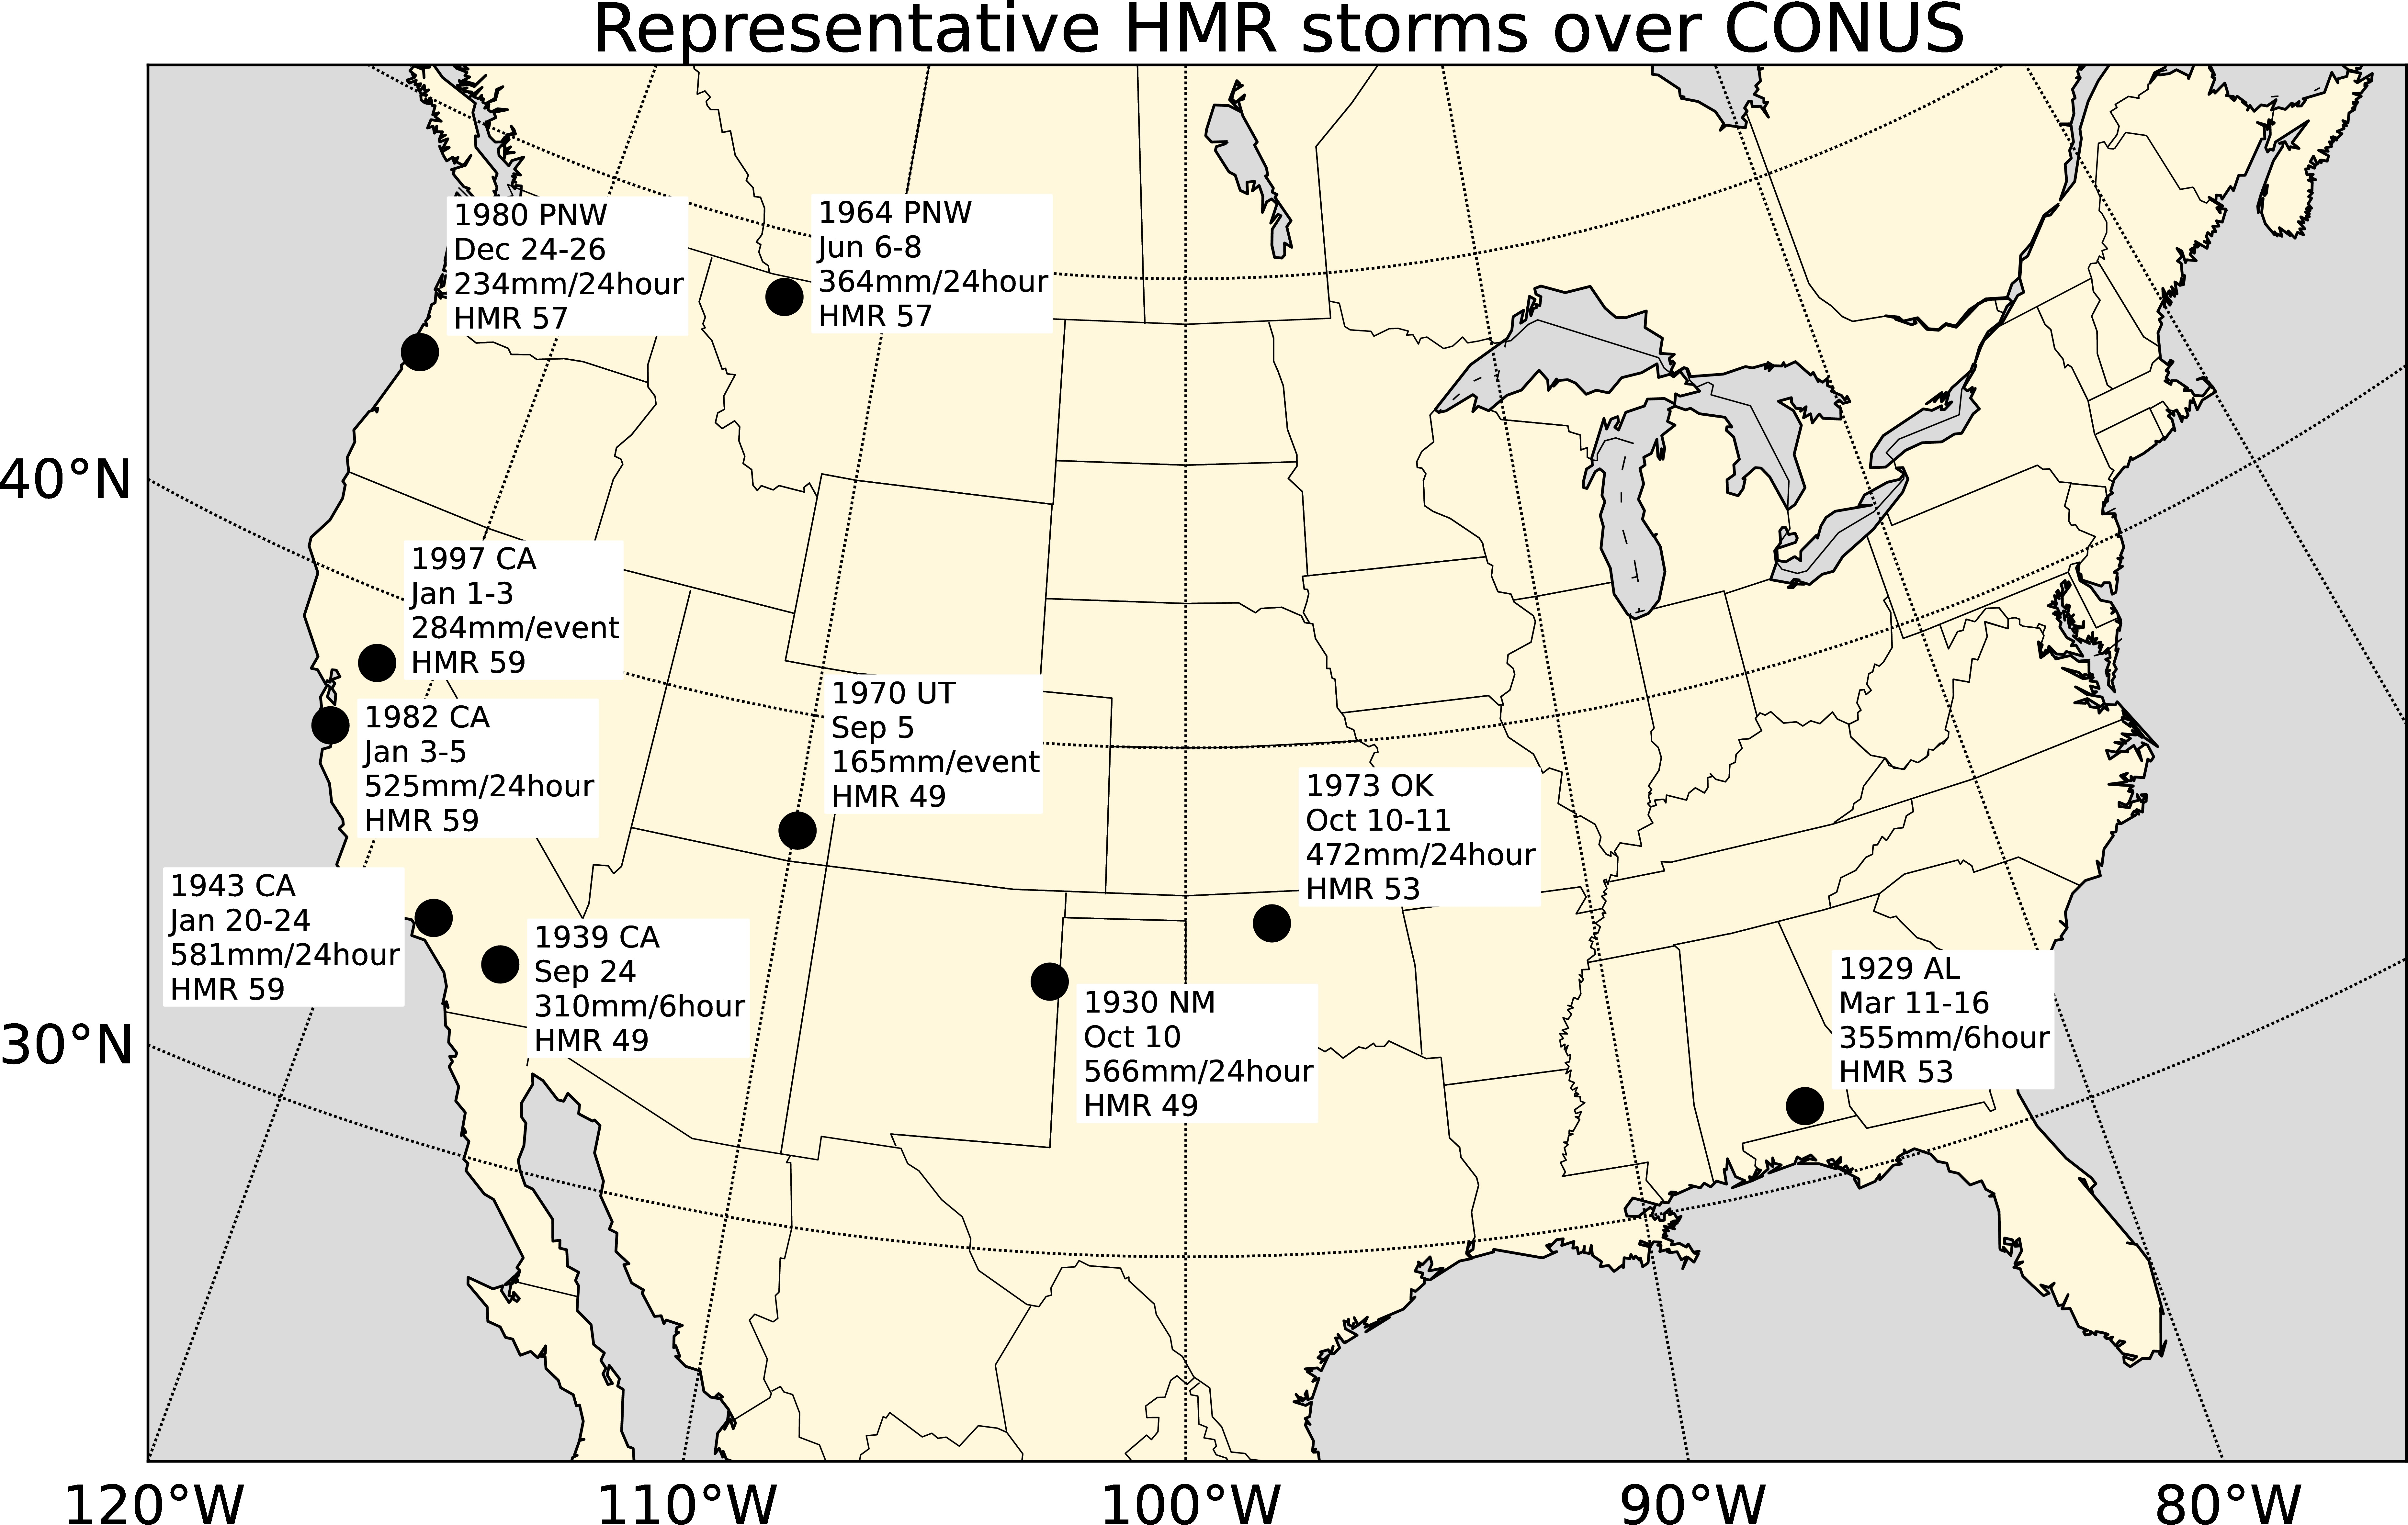
\includegraphics[width=\linewidth]{pics/ch3/fig1.jpg}
	\caption{Location of 10 representative extreme storms in Chapter 3.}
	\label{fig:3-1}
\end{figure}


\begin{table}[htbp]
	\centering
	\caption{Basic information of the 10 representative storms in Chapter 3.}
	\begin{tabular}{cccccc}
		\hline
		%Storm ID  &  Dates  & HMR region  & \multicolumn{1}{p{2cm}}{Representative location}  & Duration  & \multicolumn{1}{p{3cm}}{\ Maximum point rainfall (mm)}\\
		\multirow{2}{*}{Storm ID} & \multirow{2}{*}{Dates} & HMR & Representative & \multirow{2}{*}{Duration} & Maximum point\\
		& & region & location & & rainfall (mm)\\
		\hline
		1997-CA  & Jan.1-3,1997   & 59 & ($38.60^{\circ}$N, $121.50^{\circ}$W) & 24 hours & 284\\
		1982-CA  & Jan.3-5,1982   & 59 & ($37.08^{\circ}$N, $122.02^{\circ}$W) & 24 hours & 525\\
		1980-PNW & Dec.24-26,1980 & 57 & ($44.92^{\circ}$N, $123.73^{\circ}$W) & 24 hours & 234\\
		1973-OK  & Oct.10-11,1973 & 53 & ($36.42^{\circ}$N, $97.87^{\circ}$W)  & 24 hours & 472\\
		1970UT   & Sep.5,1970     & 49 & ($37.63^{\circ}$N, $109.92^{\circ}$W) & Event    & 165\\
		1964-PNW & Jun.6-8,1964   & 57 & ($48.58^{\circ}$N, $113.38^{\circ}$W) & 24 hours & 364\\
		1943-CA  & Jan.20-24,1943 & 59 & ($34.20^{\circ}$N, $118.05^{\circ}$W) & 24 hours & 581\\
		1939-CA  & Sep.24,1939    & 49 & ($33.72^{\circ}$N, $116.23^{\circ}$W) & 6 hours  & 310\\
		1930-NM  & Oct.10,1930    & 49 & ($35.22^{\circ}$N, $103.28^{\circ}$W) & 24 hours & 566\\
		1929-AL  & Mar.11-16,1929 & 53 & ($31.42^{\circ}$N, $86.07^{\circ}$W)  & 6 hours  & 355\\
		\hline
		
	\end{tabular}
	\label{table:3-1}
\end{table}

Each rainfall event was caused by varying meteorological phenomena, and belongs to different classes of storm. The 1997-CA rainfall event was caused by an atmospheric river originating from the Hawaiian tropical region that penetrated the west coast [\textit{Tan}, 2010]. The 1982-CA rainfall event was caused by an extra-tropical cyclone that was accompanied by an atmospheric river [\textit{Ellen and Wieczorek}, 1988]. The 1973-OK rainfall event set the Oklahoma state record of daily rainfall. The tornado during this event led to the ``Enid Flood" in the following few days [\textit{Chang}, 1998]. The 1970-UT rainfall event was caused by the tropical storm ``Norma", which developed off the coast of Mexico and moved all the way to California. The 1964-PNW rainfall event was caused by one of the greatest low pressure system in the Pacific Northwest recorded since 1950. The 1939-CA rainfall event was among the 4 tropical storms that affected southern California during September 1939, and it was one of very few events in the Pacific Ocean with the tropical storm that actually hit the coast. The 1929-AL rainfall event was among a series of heavy rainfall events that occurred in February-March 1929, and it caused one of the worst flood events in Alabama’s history at Elba [\textit{Bullard}, 2008].

\subsection{The numerical atmospheric model}

The numerical model used for reconstruction of historical storms is the Weather Research and Forecasting (WRF) model. WRF is an atmospheric numerical modeling system widely used in operations and research. WRF has demonstrated its capability of constructing the atmospheric activities at both event-scale and long-term scale, at both local and regional scales [\textit{Skamarock et al.}, 2005]. It is developed through a multi-institute collaboration led by the National Center for Atmospheric Research (NCAR) and National Oceanic and Atmospheric Administration (NOAA). The model uses Arakawa-C horizontal grids and uses the non-hydrostatic equations for atmospheric dynamics representation [\textit{Skamarock et al.}, 2005].
During its continuous development, WRF has incorporated several advances in atmospheric sciences. This flexible framework allows for different parameterization options to be considered for various processes, such as cloud microphysics process, cumulus processes, planetary boundary process and land surface process.

\subsection{Experimental design}

Previous studies suggest that WRF performance is mostly affected by the choices of cloud microphysics and cumulus parameterization schemes [\textit{Stensrud}, 2009; \textit{Kumar et al.}, 2008; \textit{Chang et al.}, 2009]. Model resolution and initial/boundary conditions (IC/BC) also affect the simulation quality [\textit{Rajeevan et al.}, 2010; \textit{Liu et al.}, 2012]. The model configurations are inherited from study by Chen et al. (2016). Specifically, we test 3 different cloud microphysics schemes: 1) Morrison scheme, denoted as ``M"; 2) new Thompson scheme, ``T"; 3) WSM-5 scheme, ``W", and 3 cumulus schemes: 1) Kain-Fritsch (new Eta) scheme, ``KF"; 2) Grell-Devenyi scheme, ``GD"; 3) Grell-Freitas scheme, ``GF". For the IC/BC in the simulation, NCEP/DOE Reanalysis II product (NCEP2) is used for storms after 1979, NCEP/NCAR reanalysis project (NNRP) is used for storms between 1948 and 1979, and NOAA-CIRES Twentieth Century Reanalysis Product (20CR) is used in simulations before 1948. Also previous studies [\textit{Chen et al.}, 2016] suggest that for big storms, finer resolution does not always improve the simulation quality. Thus, for these 10 storms, we test 2 spatial resolutions: 1) single 15km domain; 2) two-way nested 15km-5km domain. Model configuration is coded as ``gX-Y-Z", in which X is the resolution, Y is the microphysics scheme, and Z is the cumulus scheme. For example, ``g5-W-GF" means a 15km-5km nested run using WSM-5 microphysics and Grell-Freitas cumulus schemes. Further explanation of these configuration codes is provided in Table \ref{table:3-S1}. The simulation durations are chosen to include the storm duration until complete dissipation, with 1 extra day in the beginning to spin up the model. Simulation durations are summarized in Table \ref{table:3-S2}.

The evaluation of WRF simulated precipitation was done using Livneh daily CONUS near-surface gridded meteorological dataset [\textit{Livneh et al.}, 2013]. This precipitation data was generated from rain gauge records since 1915, and it is one of the very few long-term precipitation data over CONUS. The evaluation consists of two parts: 1) Evaluation of the spatial coverage of daily rainfall. This is done under the various metrics (Probability of Detection, $POD$; False Alert Ratio, $FAR$; Frequency Bias, $Bias$; Heidke Skill Score, $HSS$; Critical Score Index, $CSI$), and their definitions are shown in Chapter 2; 2) Evaluation of storm statistical characteristics. Because PMP is defined as the maximum probable rainfall in a given duration, it is useful to check the simulated temporal structure of the storms, as well as the maximum rainfall in some specified durations. This evaluation involves the correlation between the simulated rainfall and reference rainfall (Livneh data) as daily rainfall, maximum 1-day, 2-day and 3-day rainfall.


\section{Results}

To make the WRF results comparable to the Livneh dataset, all the WRF results were first conservatively regridded to the 1/16 degree ($\scriptsize{\sim}$ 8km) grids, which is the native resolution of Livneh dataset.

\subsection{Spatial coverage of rainy area}

The ability to reproduce correct rainy areas is useful in some engineering practice, such as preventive migration before the storm/flood events. Also, this shows the vulnerable areas under big storms from an infrastructure damage and flash flood perspective, where extra attention should be paid sometimes.

\begin{figure}[htbp]
	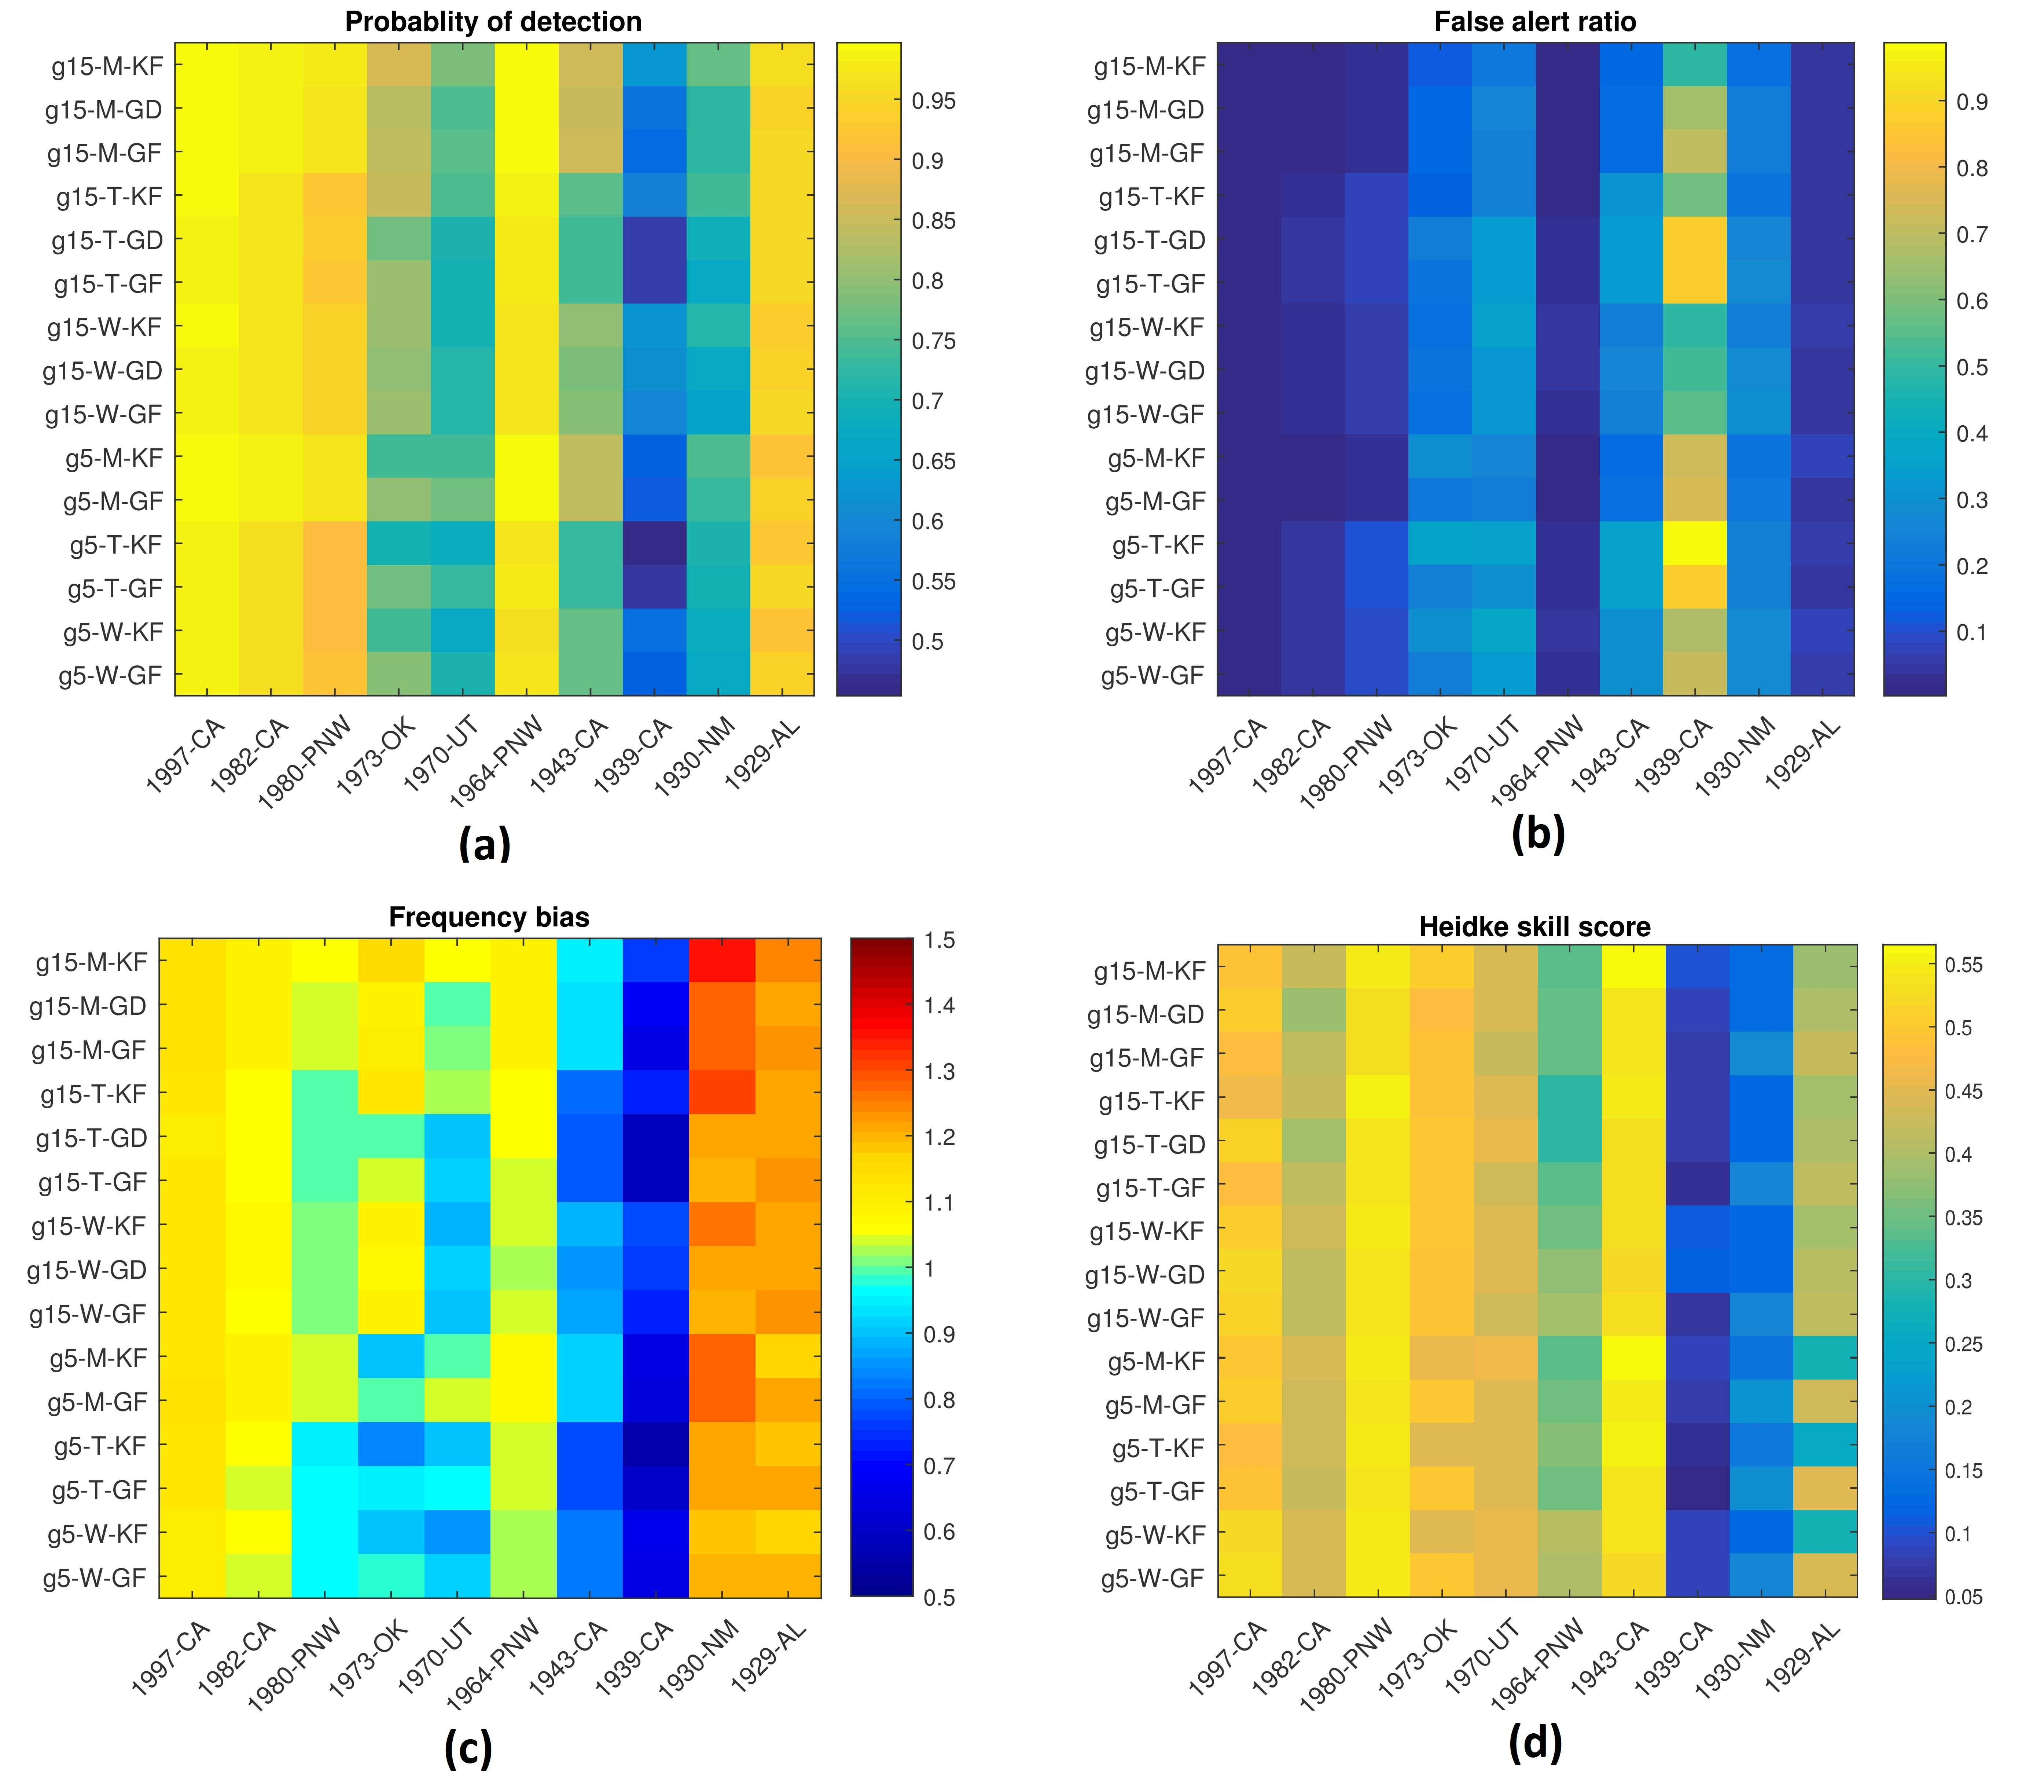
\includegraphics[width=\linewidth]{pics/ch3/fig2.jpg}
	\caption{Evaluation of reconstructed big storms: spatial coverages. Panel (a) shows the probability of detection; (b) shows the false alert ratio; (c) is the frequency bias; (d) is the Heidke skill score. The panels (abc) were computed using 0mm/day rainfall threshold (any rainy grids/days were counted as rainy), panel (d) were computed using 5mm/day threshold (grids/days with $>$5mm/day were counted as rainy).}
	\label{fig:3-2}
\end{figure}

The spatial coverage evaluation is done using the simulated and observed daily rainfall data. Figure \ref{fig:3-2} shows the calculated $POD$, $FAR$, $Bias$ and $HSS$ scores of these 10 storms using all the 15 model configurations. In these panels, x-axis shows 10 storms, from the recent ones to the older ones; y-axis shows the different model configurations, as coded in section 3.2.3. Panel \ref{fig:3-2}(a) shows the $POD$ scores, where higher scores indicate better coverage of rainy areas. Panel \ref{fig:3-2}(b) shows the FAR scores, where lower scores indicate that the model yields less ``rainy area" that is actually not rainy. A good model configuration should produce higher $POD$s while lower $FAR$s. The general trend from these 2 panels is that model performance is mostly sensitive to the choice of IC/BCs: NCEP2 IC/BC generally gives out highest $POD$ and lowest $FAR$, and the difference in the 3 storms (1997-CA, 1982-CA, 1980-PNW) are very small (i.e. the POD range of 0.9038$\scriptsize{\sim}$0.9967, compared with 0.6773$\scriptsize{\sim}$0.9971 in NNRP group and 0.4538$\scriptsize{\sim}$0.9582 in 20CR group). As we move to storms that are a few decades old, the simulations become less accurate, and the simulation quality has an abrupt drop at 1940. The results are also more sensitive to the cumulus scheme choices than the microphysics scheme choices. This is in agreement with the study of Pei et al. (2014), where cumulus process was diagnosed as one of the controlling factor of precipitation patterns. In the 1982-CA storm, 1970-UT storm and 1929-AL storm, $POD$ is consistently lower when KF cumulus scheme is used, despite the use of a microphysics scheme. This might suggest that KF scheme tends to underestimate the rainfall from cumulus cloud processes during the big storms.

Panel \ref{fig:3-2}(c) shows the frequency bias in the simulations. Perfect simulations should produce frequency bias close to 1 (green band in the panel). It is obvious that simulations with NCEP2 IC/BC can reconstruct the rainy regions whose area is close to the observation. In the simulations with NNRP and 20CR IC/BC, however, the frequency biases have much larger variation (more biased underestimation or overestimation). Also simulations with NCEP2 IC/BC tend to overestimate the rainy area, while simulations with NNRP IC/BC tend to underestimate the rainy area. We will investigate this difference using histograms of daily rainfall amounts later. Panel \ref{fig:3-2}(d) shows the Heidke skill scores, which need to be larger than 0 for a model to be skillful. All these 4 metrics indicate that in all these storms, the 1939-CA case produced the worst scores. 

Table \ref{table:3-2} shows the $CSI$ scores for all WRF simulations. More recent storms experience higher $CSI$ and the high $CSI$ is maintained in the NCEP2 and NNRP IC/BC simulations. $CSI$ gradually drops as we attempt to reconstruct older storms. Among simulations using 20CR, the 1943-CA and 1929-AL cases both receive better $CSI$ scores, but the reasons are different: For the 1943-CA event, the simulated rainfall process resembles the observed process; for the 1929-AL event, however, the simulated rainfall only shares the spatial coverage with observation, while the location of the storm center is largely biased. This is obvious when we compare the maximum 3-day rainfall maps in the following section. For other storms simulated using 20CR IC/BC, the $CSI$ is low, thus 20CR is in general not a good option for stormy area reconstructions.

\begin{table}[htbp]
	\centering
	\caption{$CSI$ scores for the 10 storms}
	\begin{tabular}{ccccccccccc}
		\hline
		\multirow{2}{*}{Storm} & 1997- & 1982- & 1980- & 1973- & 1970- & 1964- & 1943- & 1939- & 1930- & 1929-\\
		& CA & CA & PNW & OK & UT & PNW & CA & CA & NM & AL\\
		\hline
		g15-M-KF & 0.879 & 0.891 & 0.904 & 0.672 & 0.610 & 0.918 & 0.798 & 0.555 & 0.480 & 0.744\\
		g15-M-GD & 0.877 & 0.893 & 0.903 & 0.661 & 0.601 & 0.919 & 0.790 & 0.500 & 0.461 & 0.746\\
		g15-M-GF & 0.877 & 0.892 & 0.903 & 0.666 & 0.602 & 0.920 & 0.791 & 0.489 & 0.462 & 0.745\\
		g15-T-KF & 0.879 & 0.883 & 0.877 & 0.671 & 0.588 & 0.908 & 0.721 & 0.520 & 0.471 & 0.751\\
		g15-T-GD & 0.873 & 0.881 & 0.879 & 0.631 & 0.584 & 0.909 & 0.703 & 0.440 & 0.448 & 0.751\\
		g15-T-GF & 0.877 & 0.881 & 0.875 & 0.649 & 0.573 & 0.908 & 0.706 & 0.436 & 0.442 & 0.748\\
		g15-W-KF & 0.878 & 0.883 & 0.881 & 0.636 & 0.577 & 0.902 & 0.741 & 0.540 & 0.459 & 0.739\\
		g15-W-GD & 0.879 & 0.883 & 0.882 & 0.625 & 0.595 & 0.904 & 0.726 & 0.532 & 0.432 & 0.737\\
		g15-W-GF & 0.880 & 0.882 & 0.883 & 0.635 & 0.592 & 0.911 & 0.732 & 0.521 & 0.426 & 0.740\\
		g5-M-KF & 0.879 & 0.891 & 0.905 & 0.638 & 0.590 & 0.916 & 0.788 & 0.473 & 0.491 & 0.730\\
		g5-M-GF & 0.879 & 0.892 & 0.904 & 0.668 & 0.605 & 0.920 & 0.784 & 0.462 & 0.471 & 0.742\\
		g5-T-KF & 0.879 & 0.879 & 0.865 & 0.610 & 0.563 & 0.903 & 0.702 & 0.413 & 0.470 & 0.740\\
		g5-T-GF & 0.878 & 0.877 & 0.865 & 0.658 & 0.587 & 0.913 & 0.695 & 0.428 & 0.461 & 0.752\\
		g5-W-KF & 0.878 & 0.876 & 0.867 & 0.633 & 0.570 & 0.902 & 0.723 & 0.493 & 0.450 & 0.734\\
		g5-W-GF & 0.877 & 0.877 & 0.870 & 0.660 & 0.586 & 0.912 & 0.721 & 0.472 & 0.438 & 0.744\\
		\hline
	\end{tabular}
	\label{table:3-2}
\end{table}

\subsection{Maximum daily and multi-daily rainfall}

Here the analysis accounts for the actual daily rainfall together with spatial information. This is to ensure that WRF-reconstructed precipitation is able to represent the storm centers and rainfall amount as observed. To make such comparison, we calculate the correlation coefficients between simulated and observed rainfall maps. Figure \ref{fig:3-3} shows the correlation coefficient between the daily rainfalls in the simulated duration (panel \ref{fig:3-3}a), between simulated and observed maximum 1-day rainfall (panel \ref{fig:3-3}b), maximum 2-day rainfall (panel \ref{fig:3-3}c), as well as maximum 3-day rainfall (panel \ref{fig:3-3}d). The scores are better when we focus more on the overall storm characteristics (maximum rainfall of a given duration) rather than spatial-temporal structures (daily rainfall series), which is indicated by the largest correlations that exceed 0.8 in panel \ref{fig:3-3}b, \ref{fig:3-3}c and \ref{fig:3-3}d. These 4 panels are quite similar, and the correlations can be classified into 3 categories according to the IC/BC inputs used. NCEP2 and NNRP IC/BC can produce sufficiently accurate rainfall estimates, while 20CR fails in the evaluation.

\begin{figure}[htbp]
	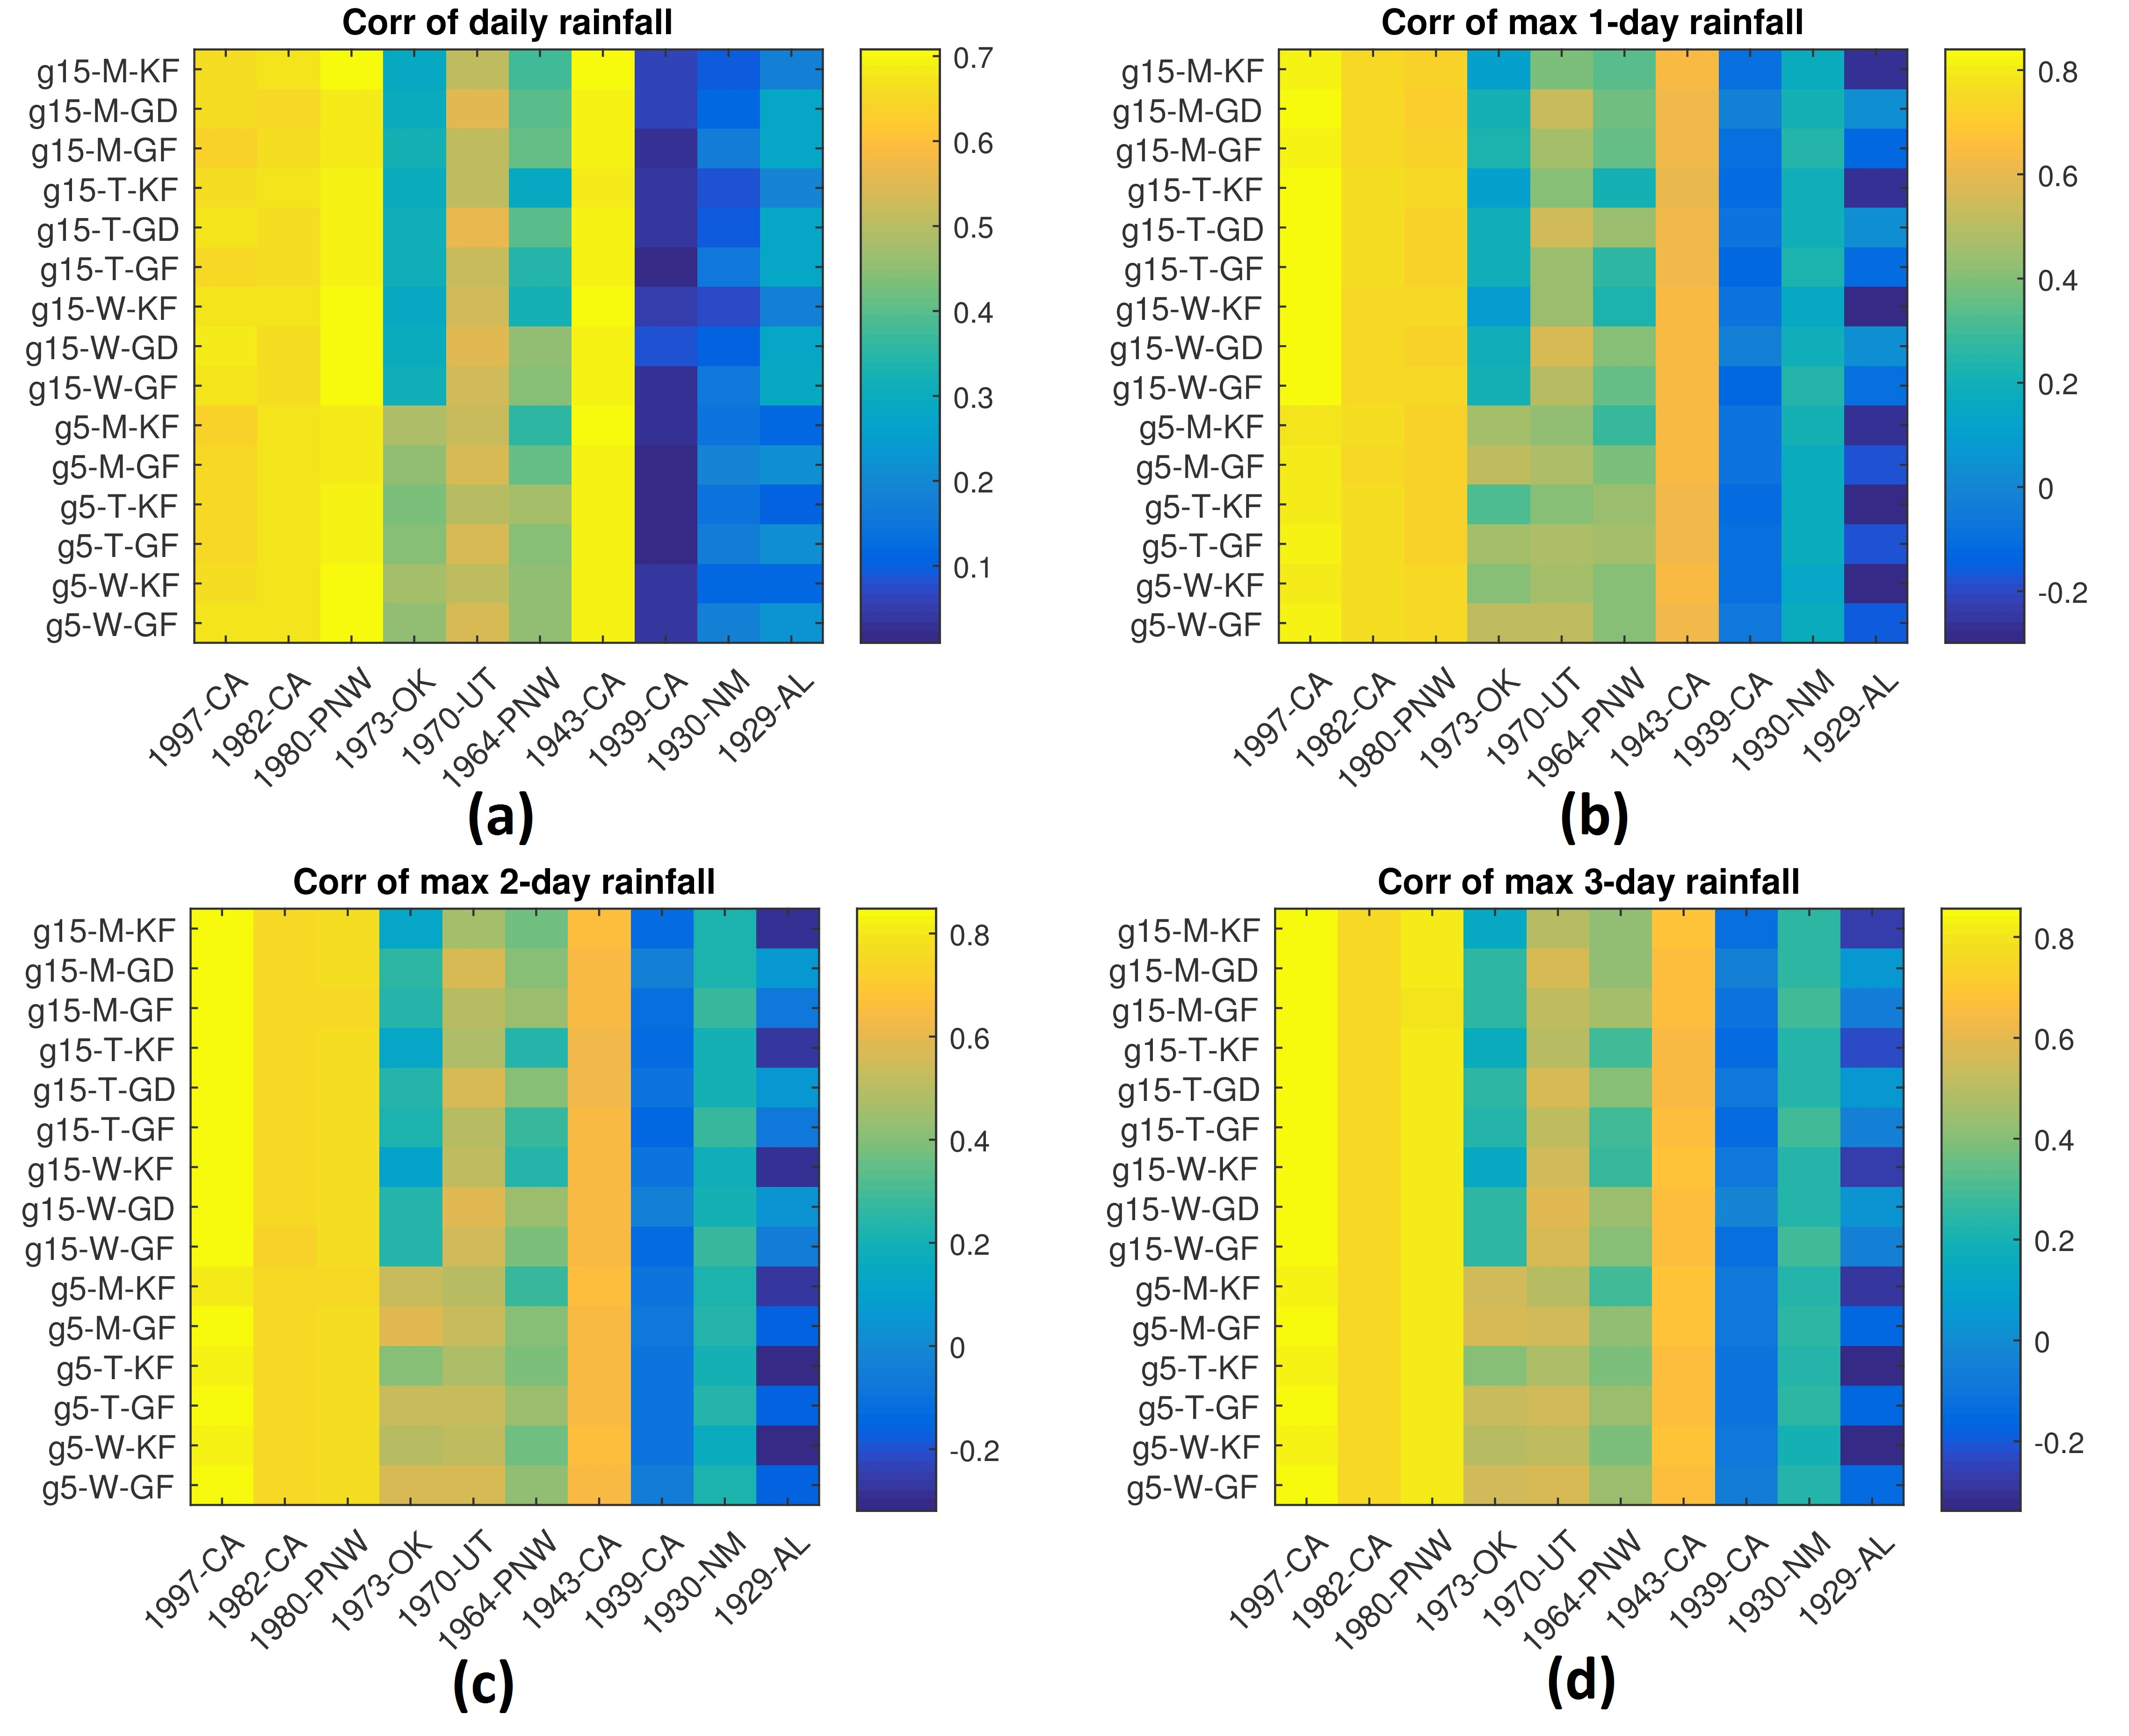
\includegraphics[width=\linewidth]{pics/ch3/fig3.jpg}
	\caption{Evaluation of reconstructed big storms: correlations with observed rainfall maps. Panel (a) show the correlation coefficient between simulated and observed daily rainfall; (b) shows the correlation between the simulated and observed maximum 1-day rainfall maps; (c) shows the correlation between the maximum 2-day rainfall maps; (d) is the correlation between the maximum 3-day rainfall maps.}
	\label{fig:3-3}
\end{figure}

The above evaluation reveals different best model configurations for these 10 storms, and they are shown in Table \ref{table:3-3}. It is obvious that the best model configuration varies from case to case. However, some similarities exist. For example, Morrison microphysics and KF cumulus schemes tend to outperform others to produce good simulations. Also the best performance is often achieved at 15km model resolution. Given that in the 15km-5km grids configuration, cumulus schemes are not used in 5km domain (except for the GF cases, where GF cumulus scheme is applied to both 15km and 5km domains), these recommendations suggest that finer grids with microphysics scheme may not necessarily resolve convective rainfall processes to the fullest extent. Thus simulating WRF with explicit cumulus parameterization scheme may still be preferred.

\begin{table}[htbp]
	\centering
	\caption{Best model configuration for the 10 storms in Chapter 3}
	\begin{threeparttable}
		\begin{tabular}{ccccc}
		\hline
		Storm & Best max 3-day rainfall corr & model resolution & Microphysics & Cumulus\\
		\hline
		1997-CA & 0.8561 & 15km & WSM-5 & GF\\
		1982-CA & 0.7546 & 5km & new Thompson & KF\\
		1980-PNW & 0.8150 & 15km & Morrison & KF\\
		1973-OK & 0.5589 & 5km & Morrison & GF\\
		1970-UT & 0.5766 & 15km & WSM-5 & GD\\
		1964-PNW & 0.4590 & 15km & Morrison & GF\\
		1943-CA & 0.6758 & 5km & Morrison & KF\\
		1939-CA & $-0.0323^{*}$ & 15km & WSM-5 & GD\\
		1930-NM & 0.2848 & 15km & Morrison & GF\\
		1929-AL & $0.0377^{**}$ & 15km & Morrison & GD\\
		\hline
		\end{tabular}
		\begin{tablenotes}
			\small
			\item $^{*}$ Correlation coefficients of max 3-day rainfall for 15 model configurations are all negative.
			\item $^{**}$ Only the shown configuration produced positive correlation coefficient.
		\end{tablenotes}
	\end{threeparttable}
	\label{table:3-3}
\end{table}

Figure \ref{fig:3-4} shows the daily rainfall correlations, max 1-day, 2-day, 3-day rainfall correlations from these configurations shown in Table \ref{table:3-2}. It suggests that with a good choice of model configuration, WRF can achieve comparable reconstruction quality for all the storms after 1940s. The correlation coefficients for these reconstructions are larger than 0.5. The reconstructions are better for more recent storms. In order to make a case of convincing PMP estimates based on numerical models under LULC and temperature change, we may need to maximize storms after 1980s for maximum skill.

\begin{figure}[htbp]
	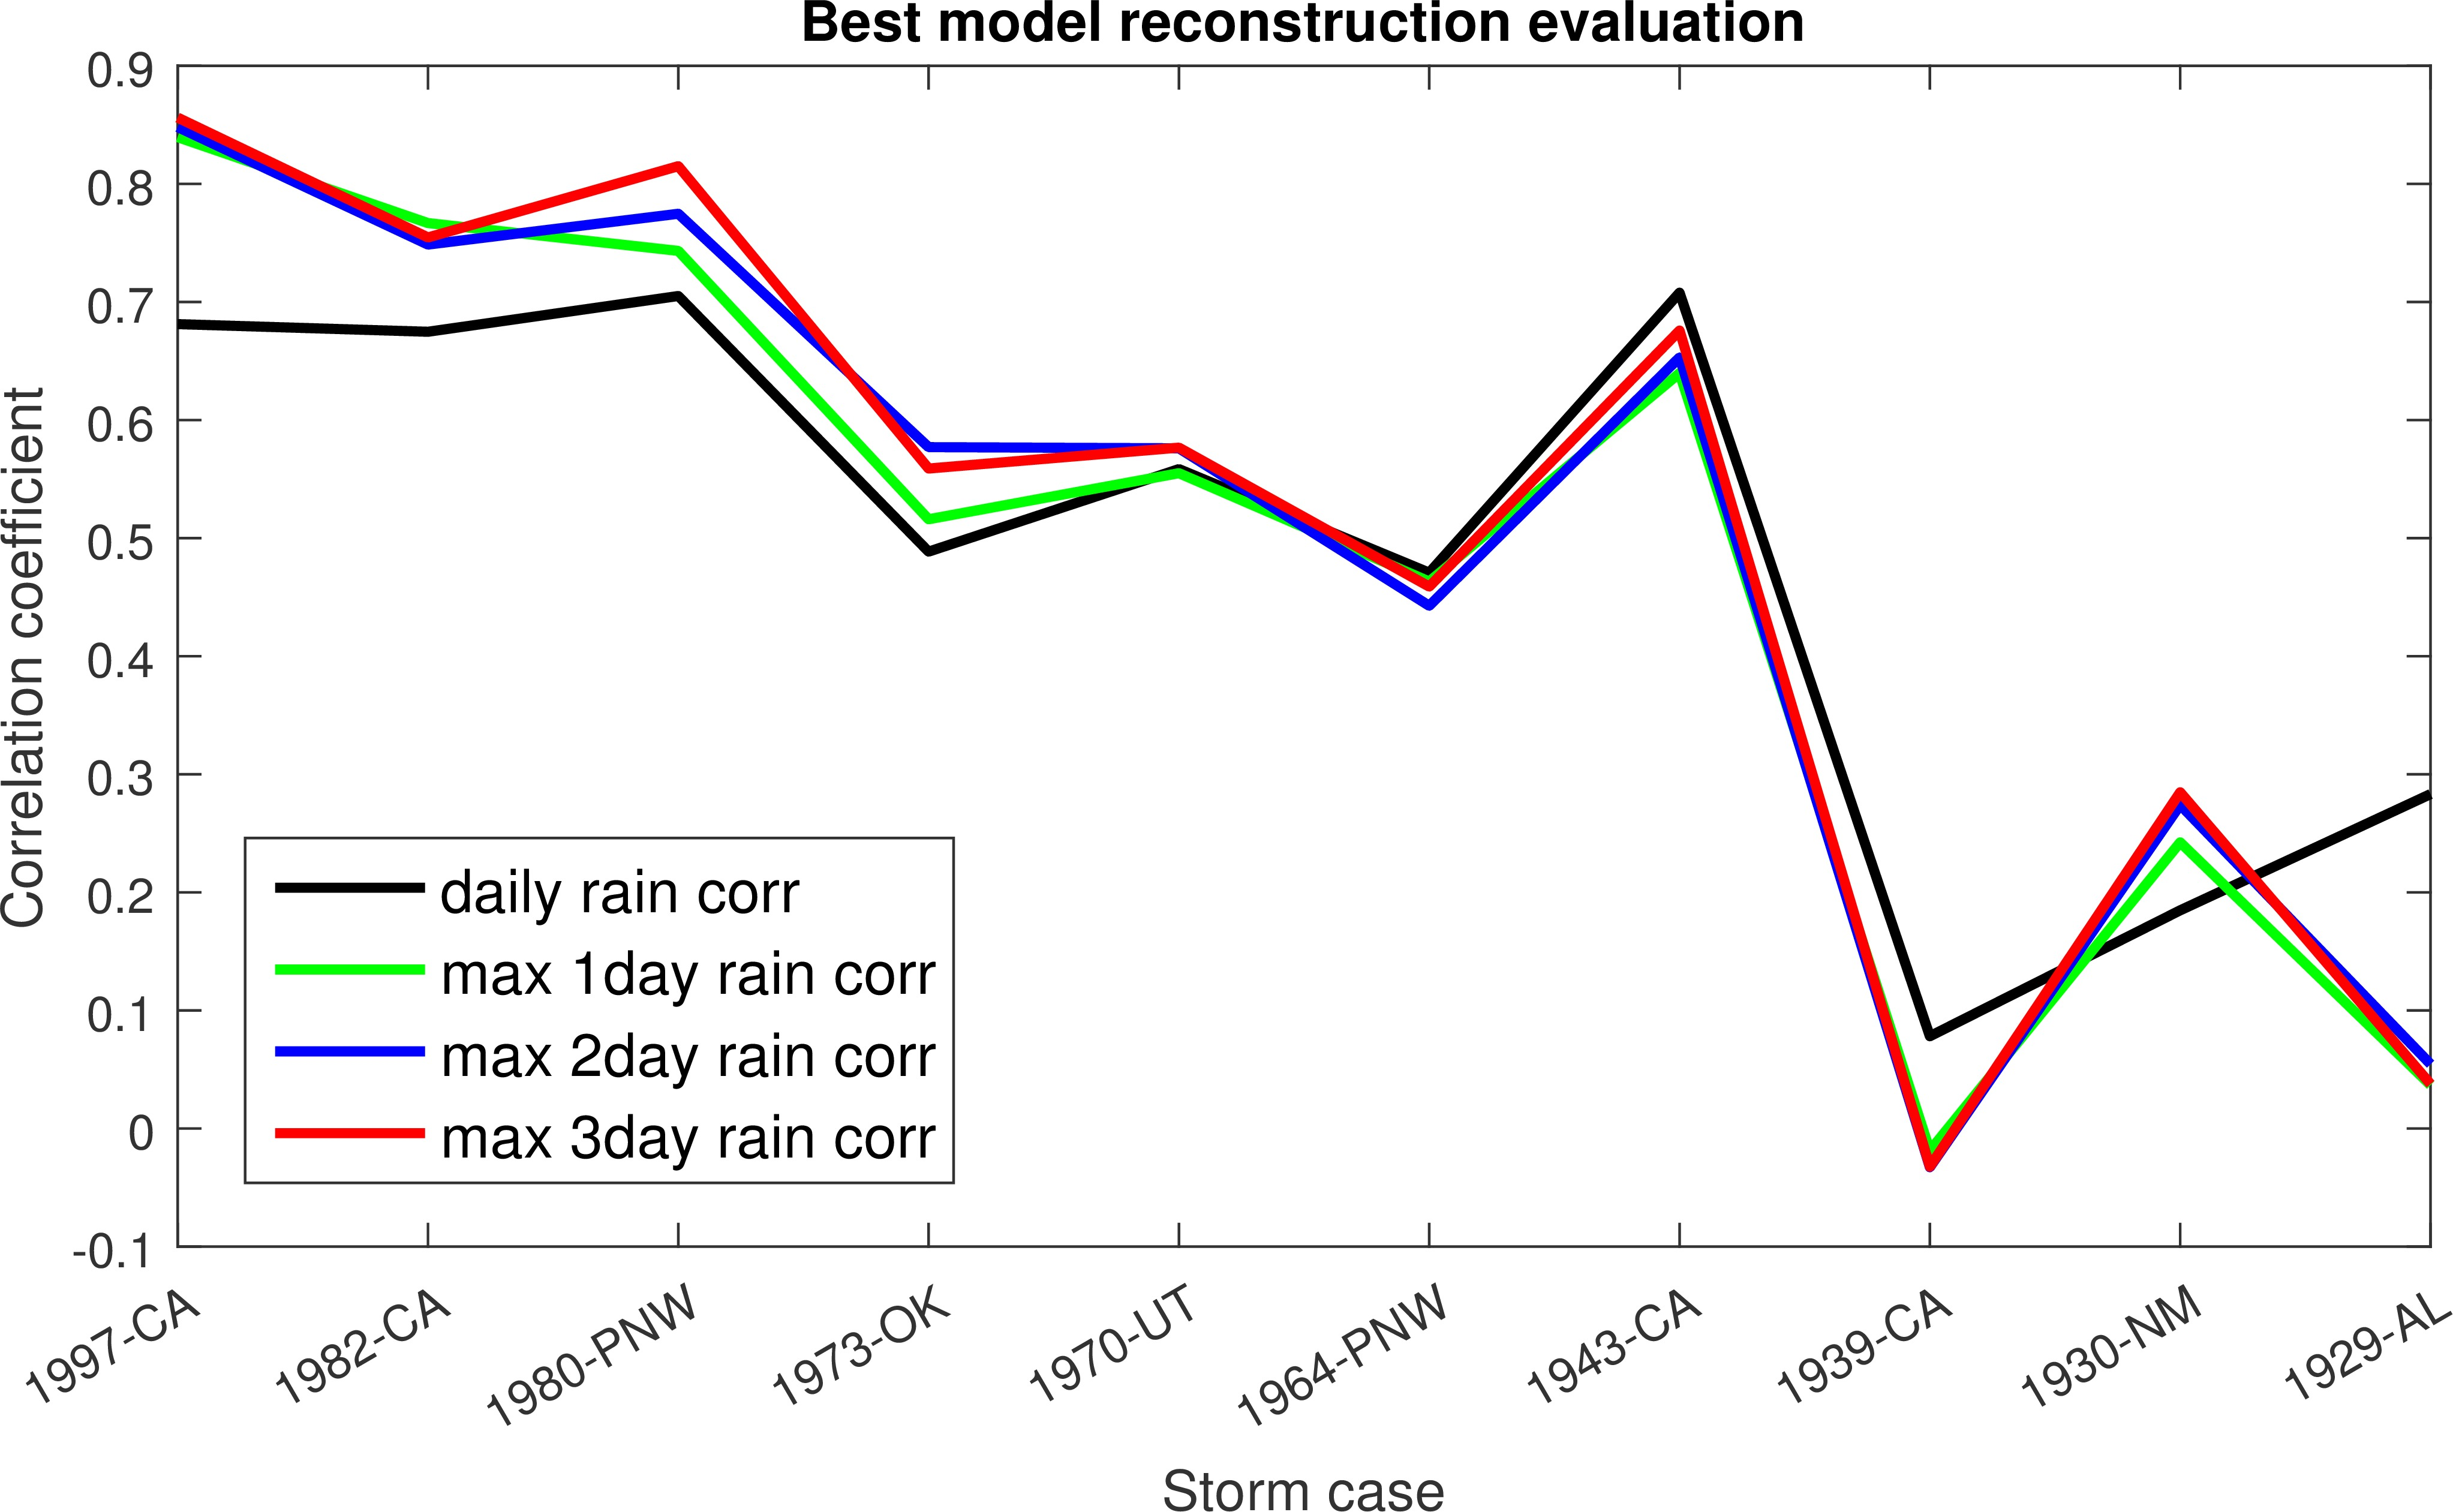
\includegraphics[width=\linewidth]{pics/ch3/fig4.jpg}
	\caption{Correlations between best reconstructions and observations.}
	\label{fig:3-4}
\end{figure}

\subsection{Maximum rainfall and duration }

Figure \ref{fig:3-5} shows the simulated and observed maximum 3-day rainfall for the 3 post-1979 storms. Figure \ref{fig:3-6} shows the same comparison of 1948-1979 storms, and figure \ref{fig:3-7} shows the comparison of pre-1948 storms.

\begin{figure}[htbp]
	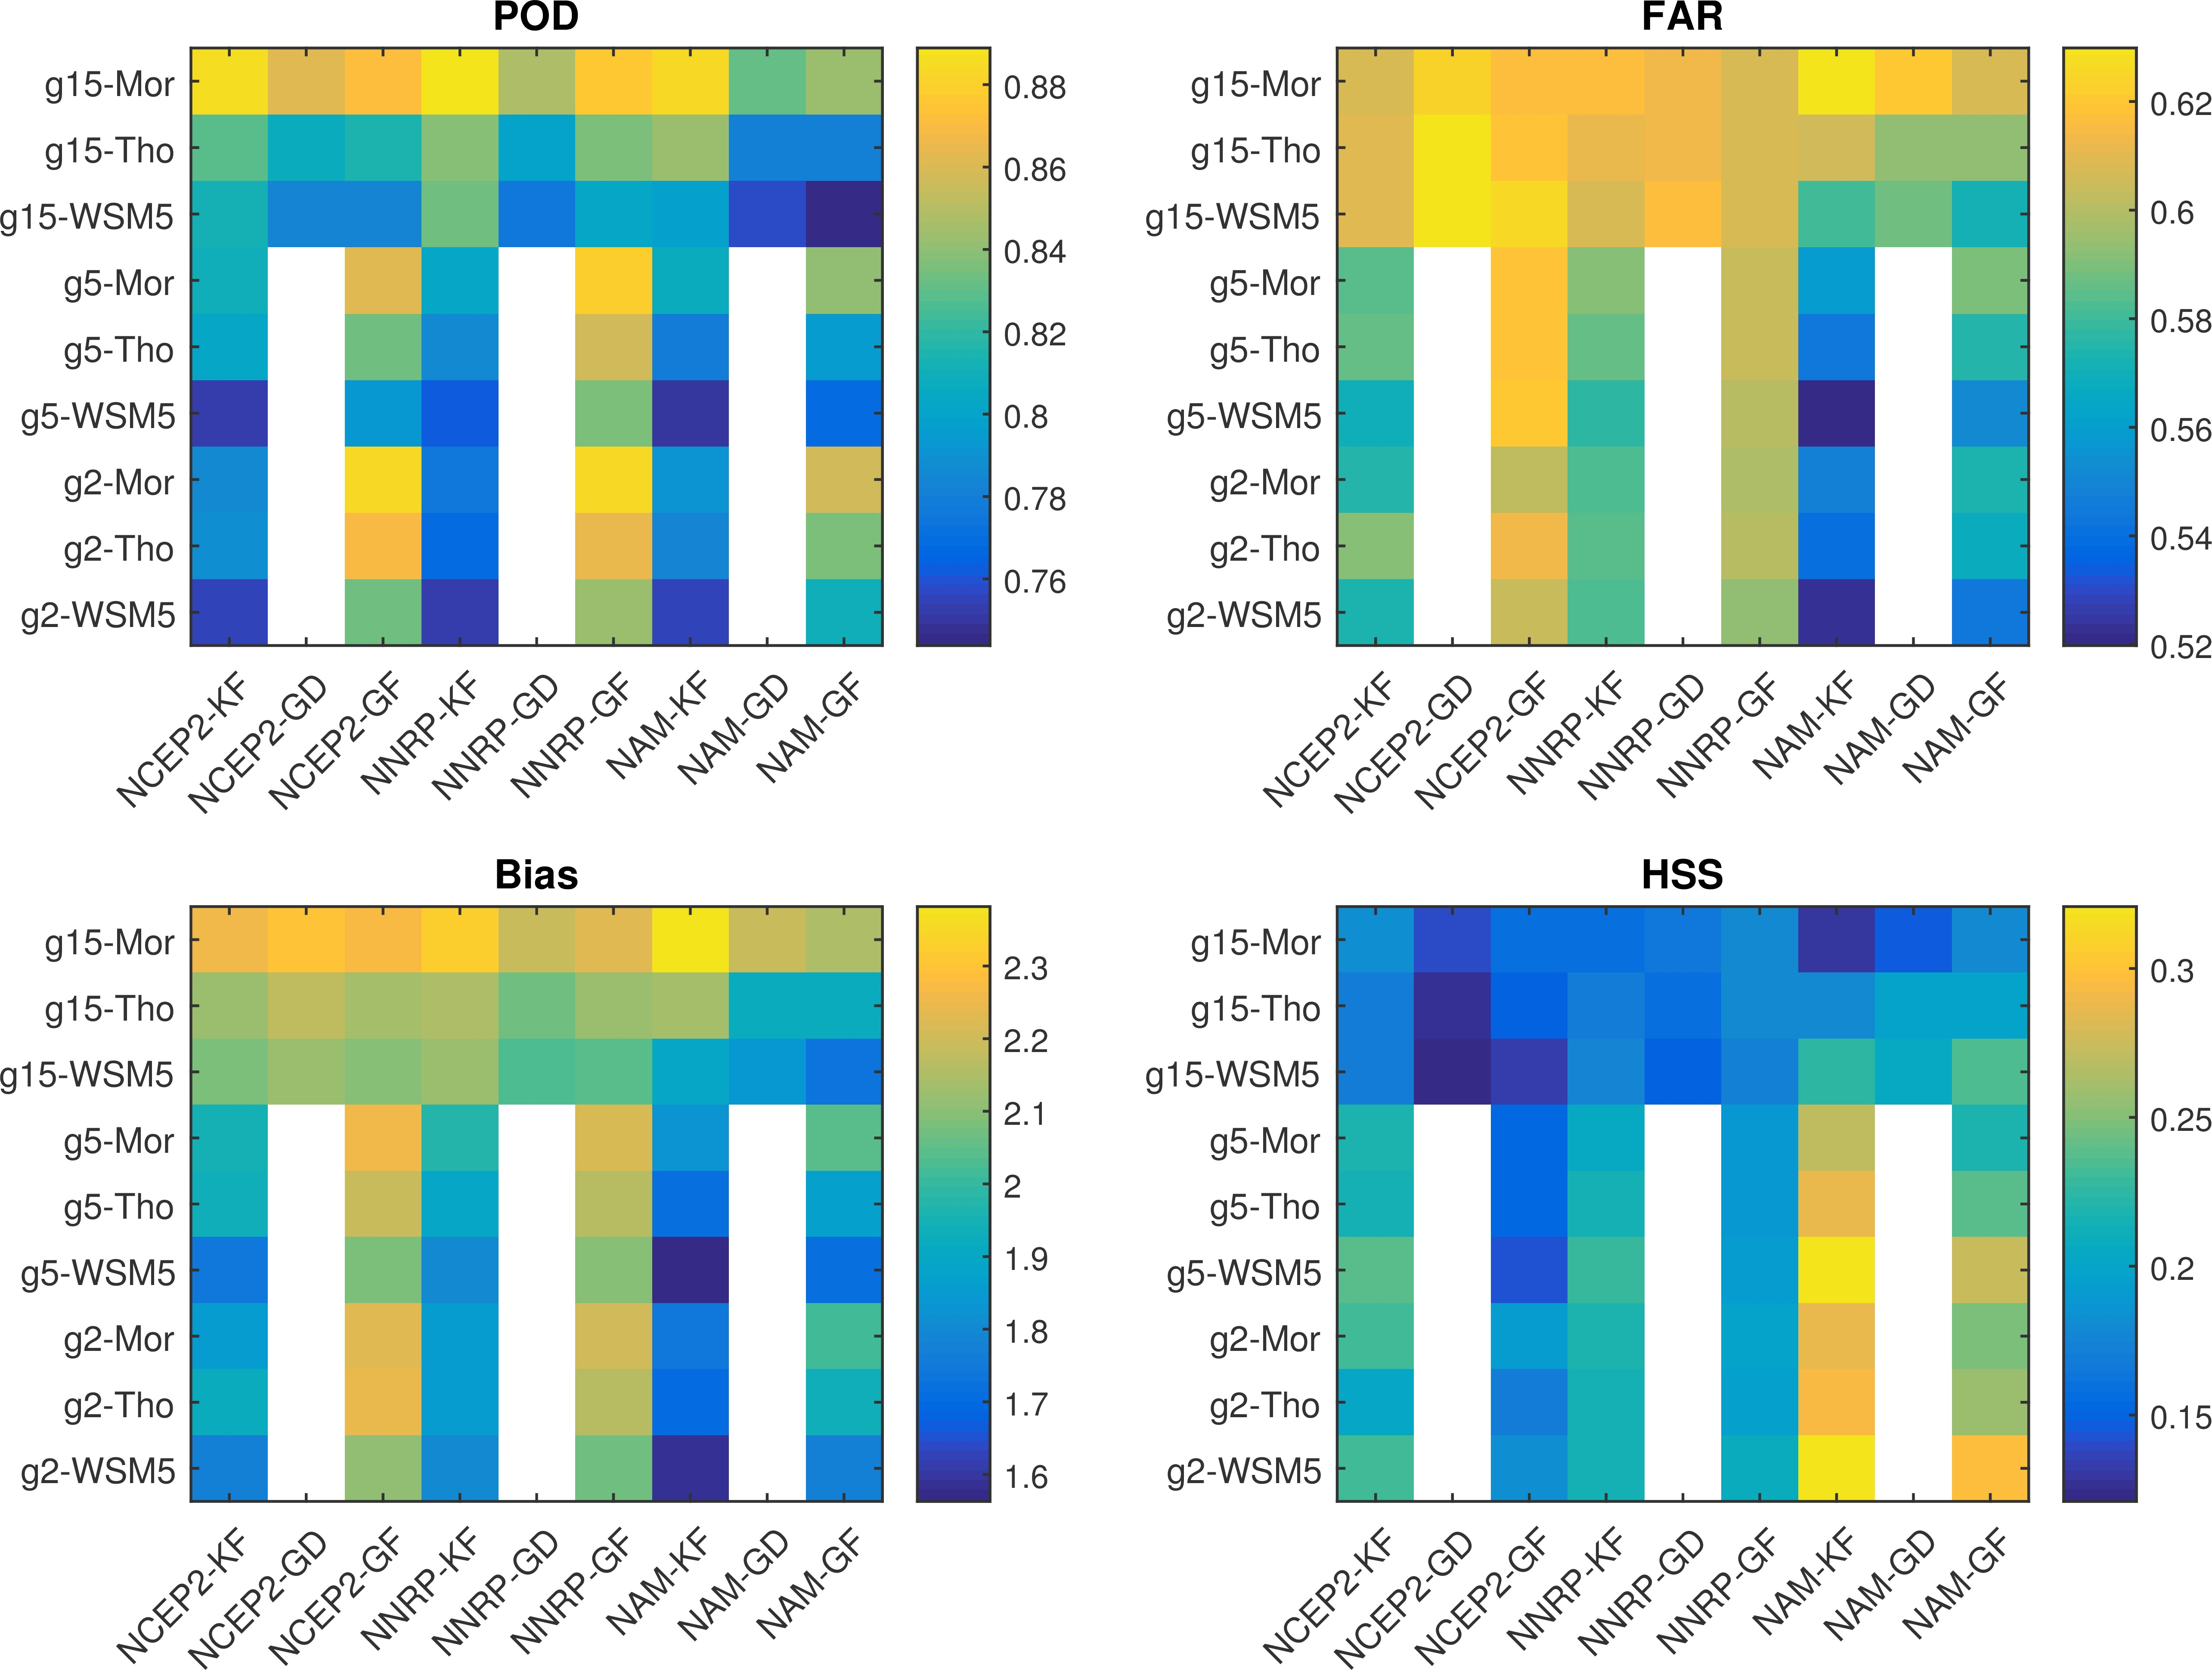
\includegraphics[width=\linewidth]{pics/ch3/fig5.jpg}
	\caption{Maximum 3-day rainfall from simulation and observation (post-1979). Panels (a,d,g) are the WRF simulation, panels (b,e,h) are the gauge observation from Livneh dataset. Panels (c,f,i) are the difference (WRF - obs). All the units are mm.}
	\label{fig:3-5}
\end{figure}

\begin{figure}[htbp]
	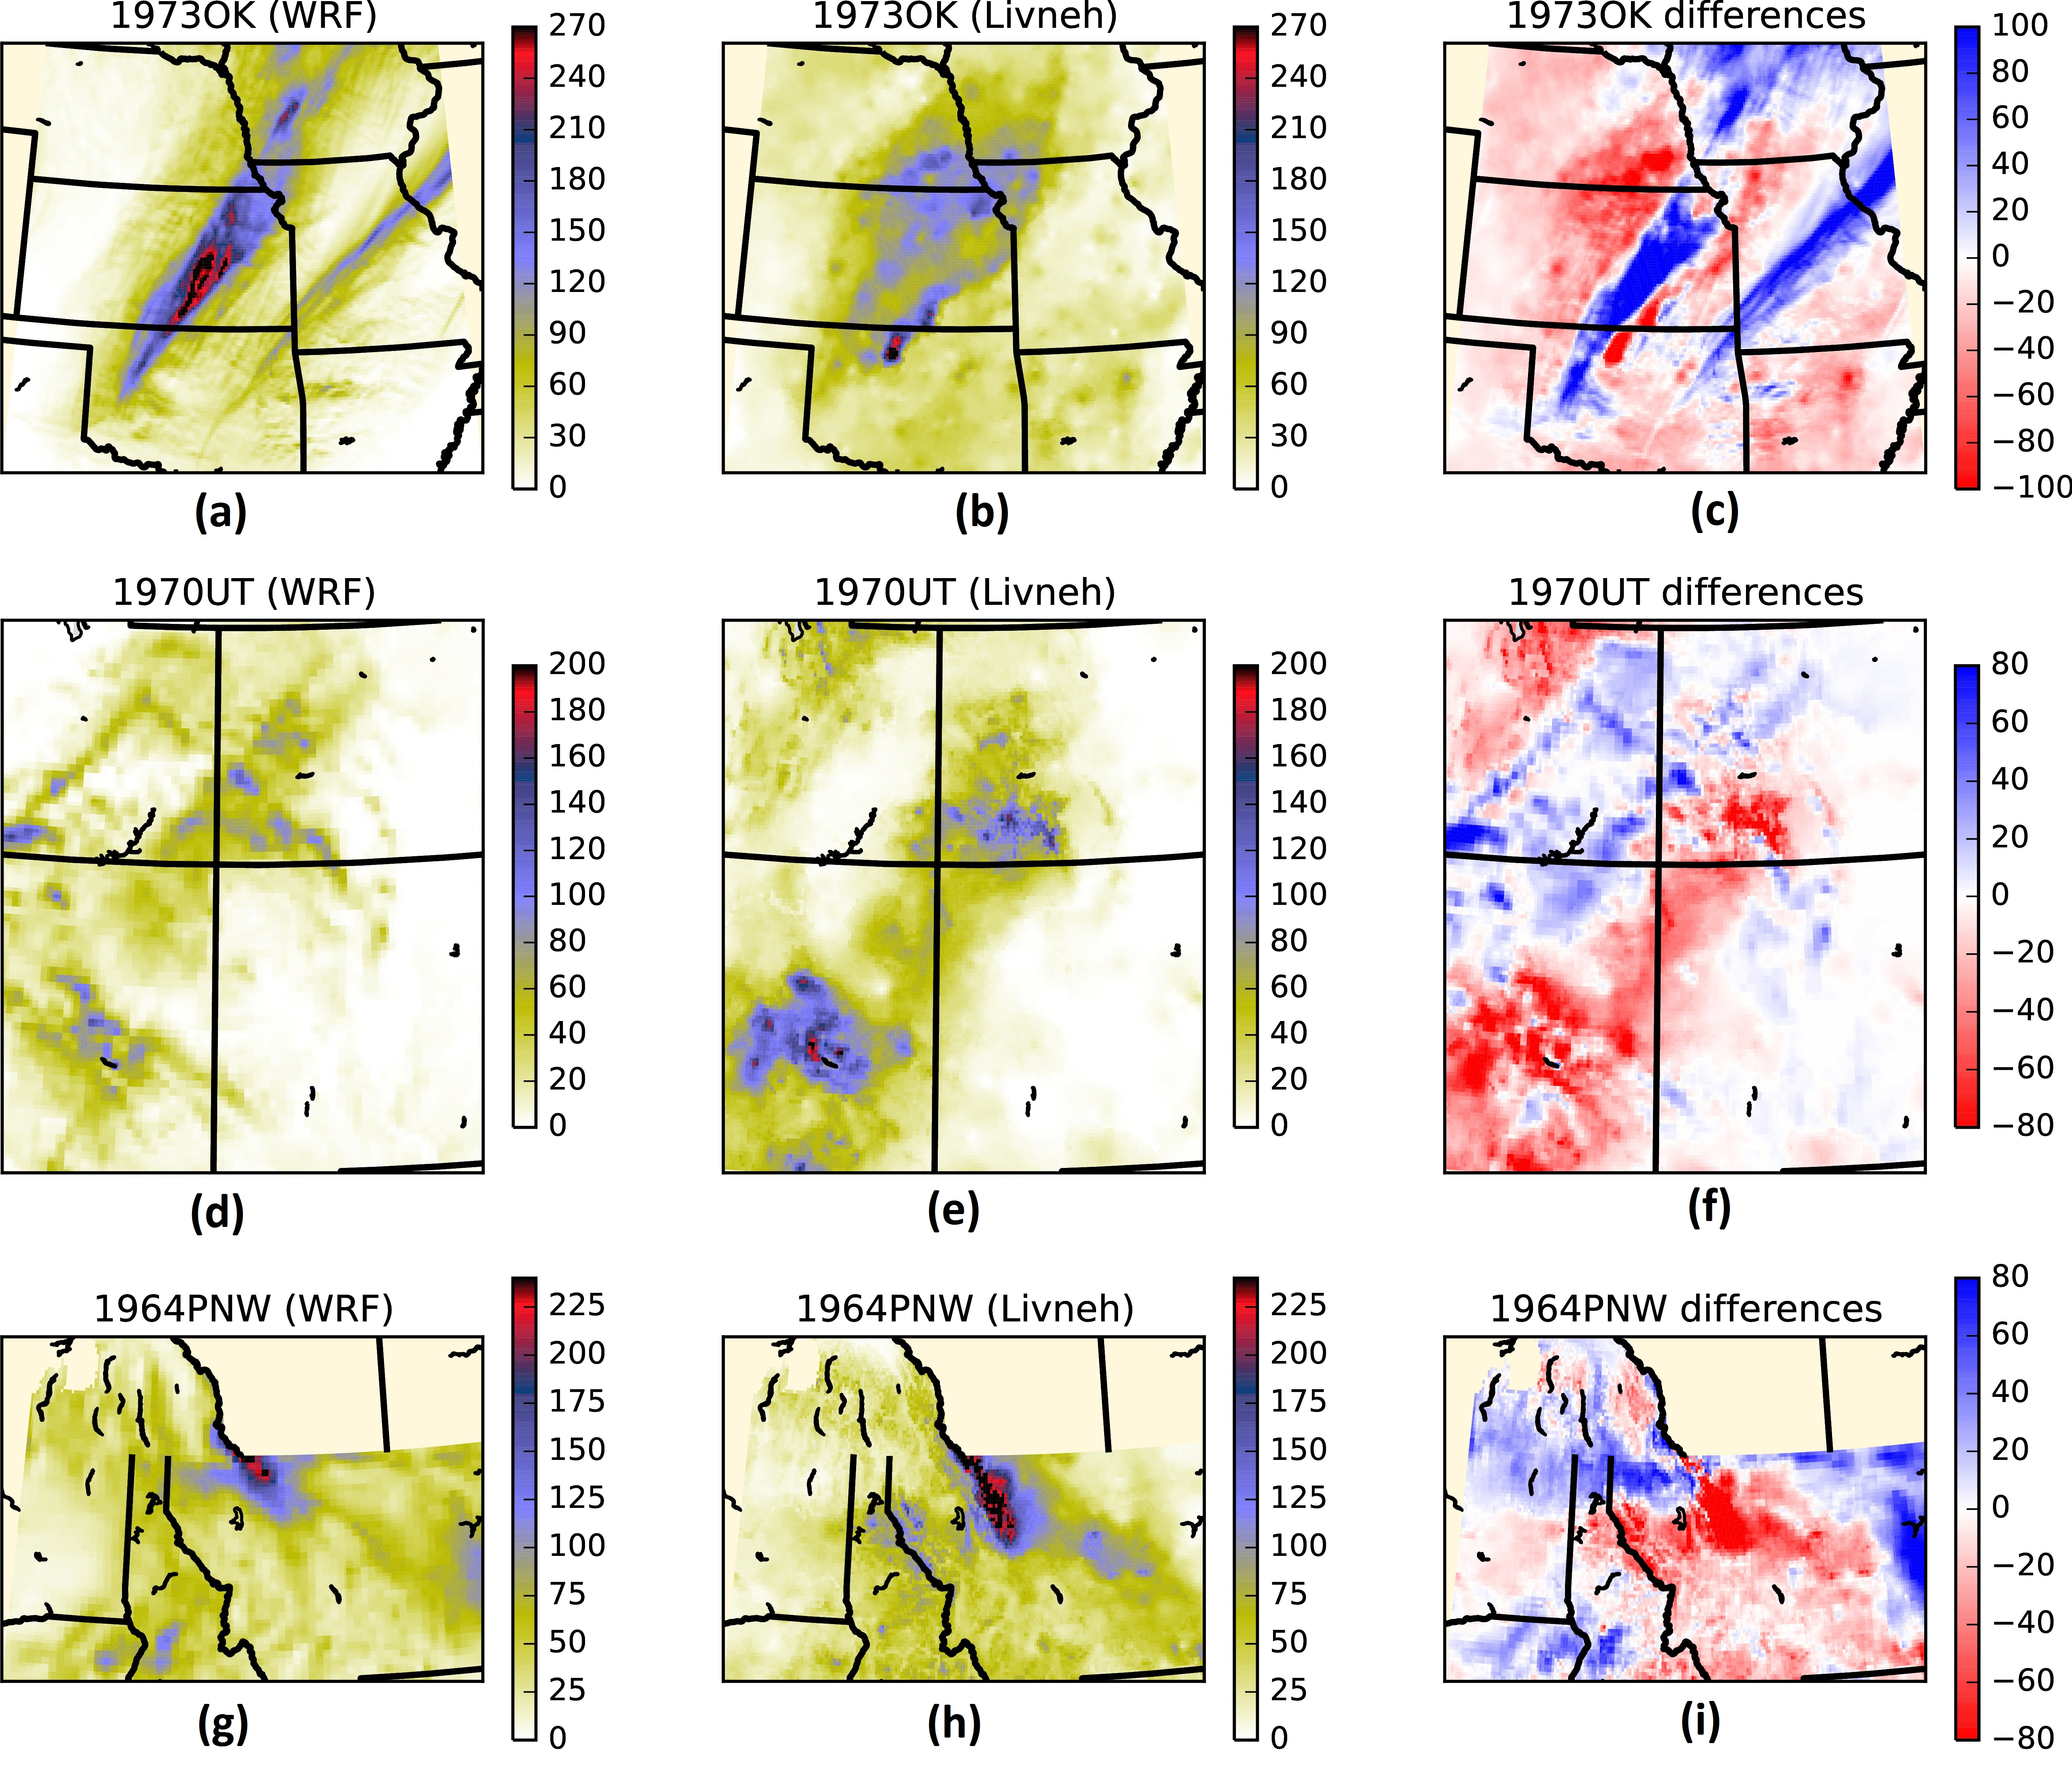
\includegraphics[width=\linewidth]{pics/ch3/fig6.jpg}
	\caption{Maximum 3-day rainfall from simulation and observation (1948-1979). Panels (a,d,g) are the WRF simulation, panels (b,e,h) are the gauge observation from Livneh dataset. Panels (c,f,i) are the difference (WRF - obs). All the units are mm.}
	\label{fig:3-6}
\end{figure}

\begin{figure}[htbp]
	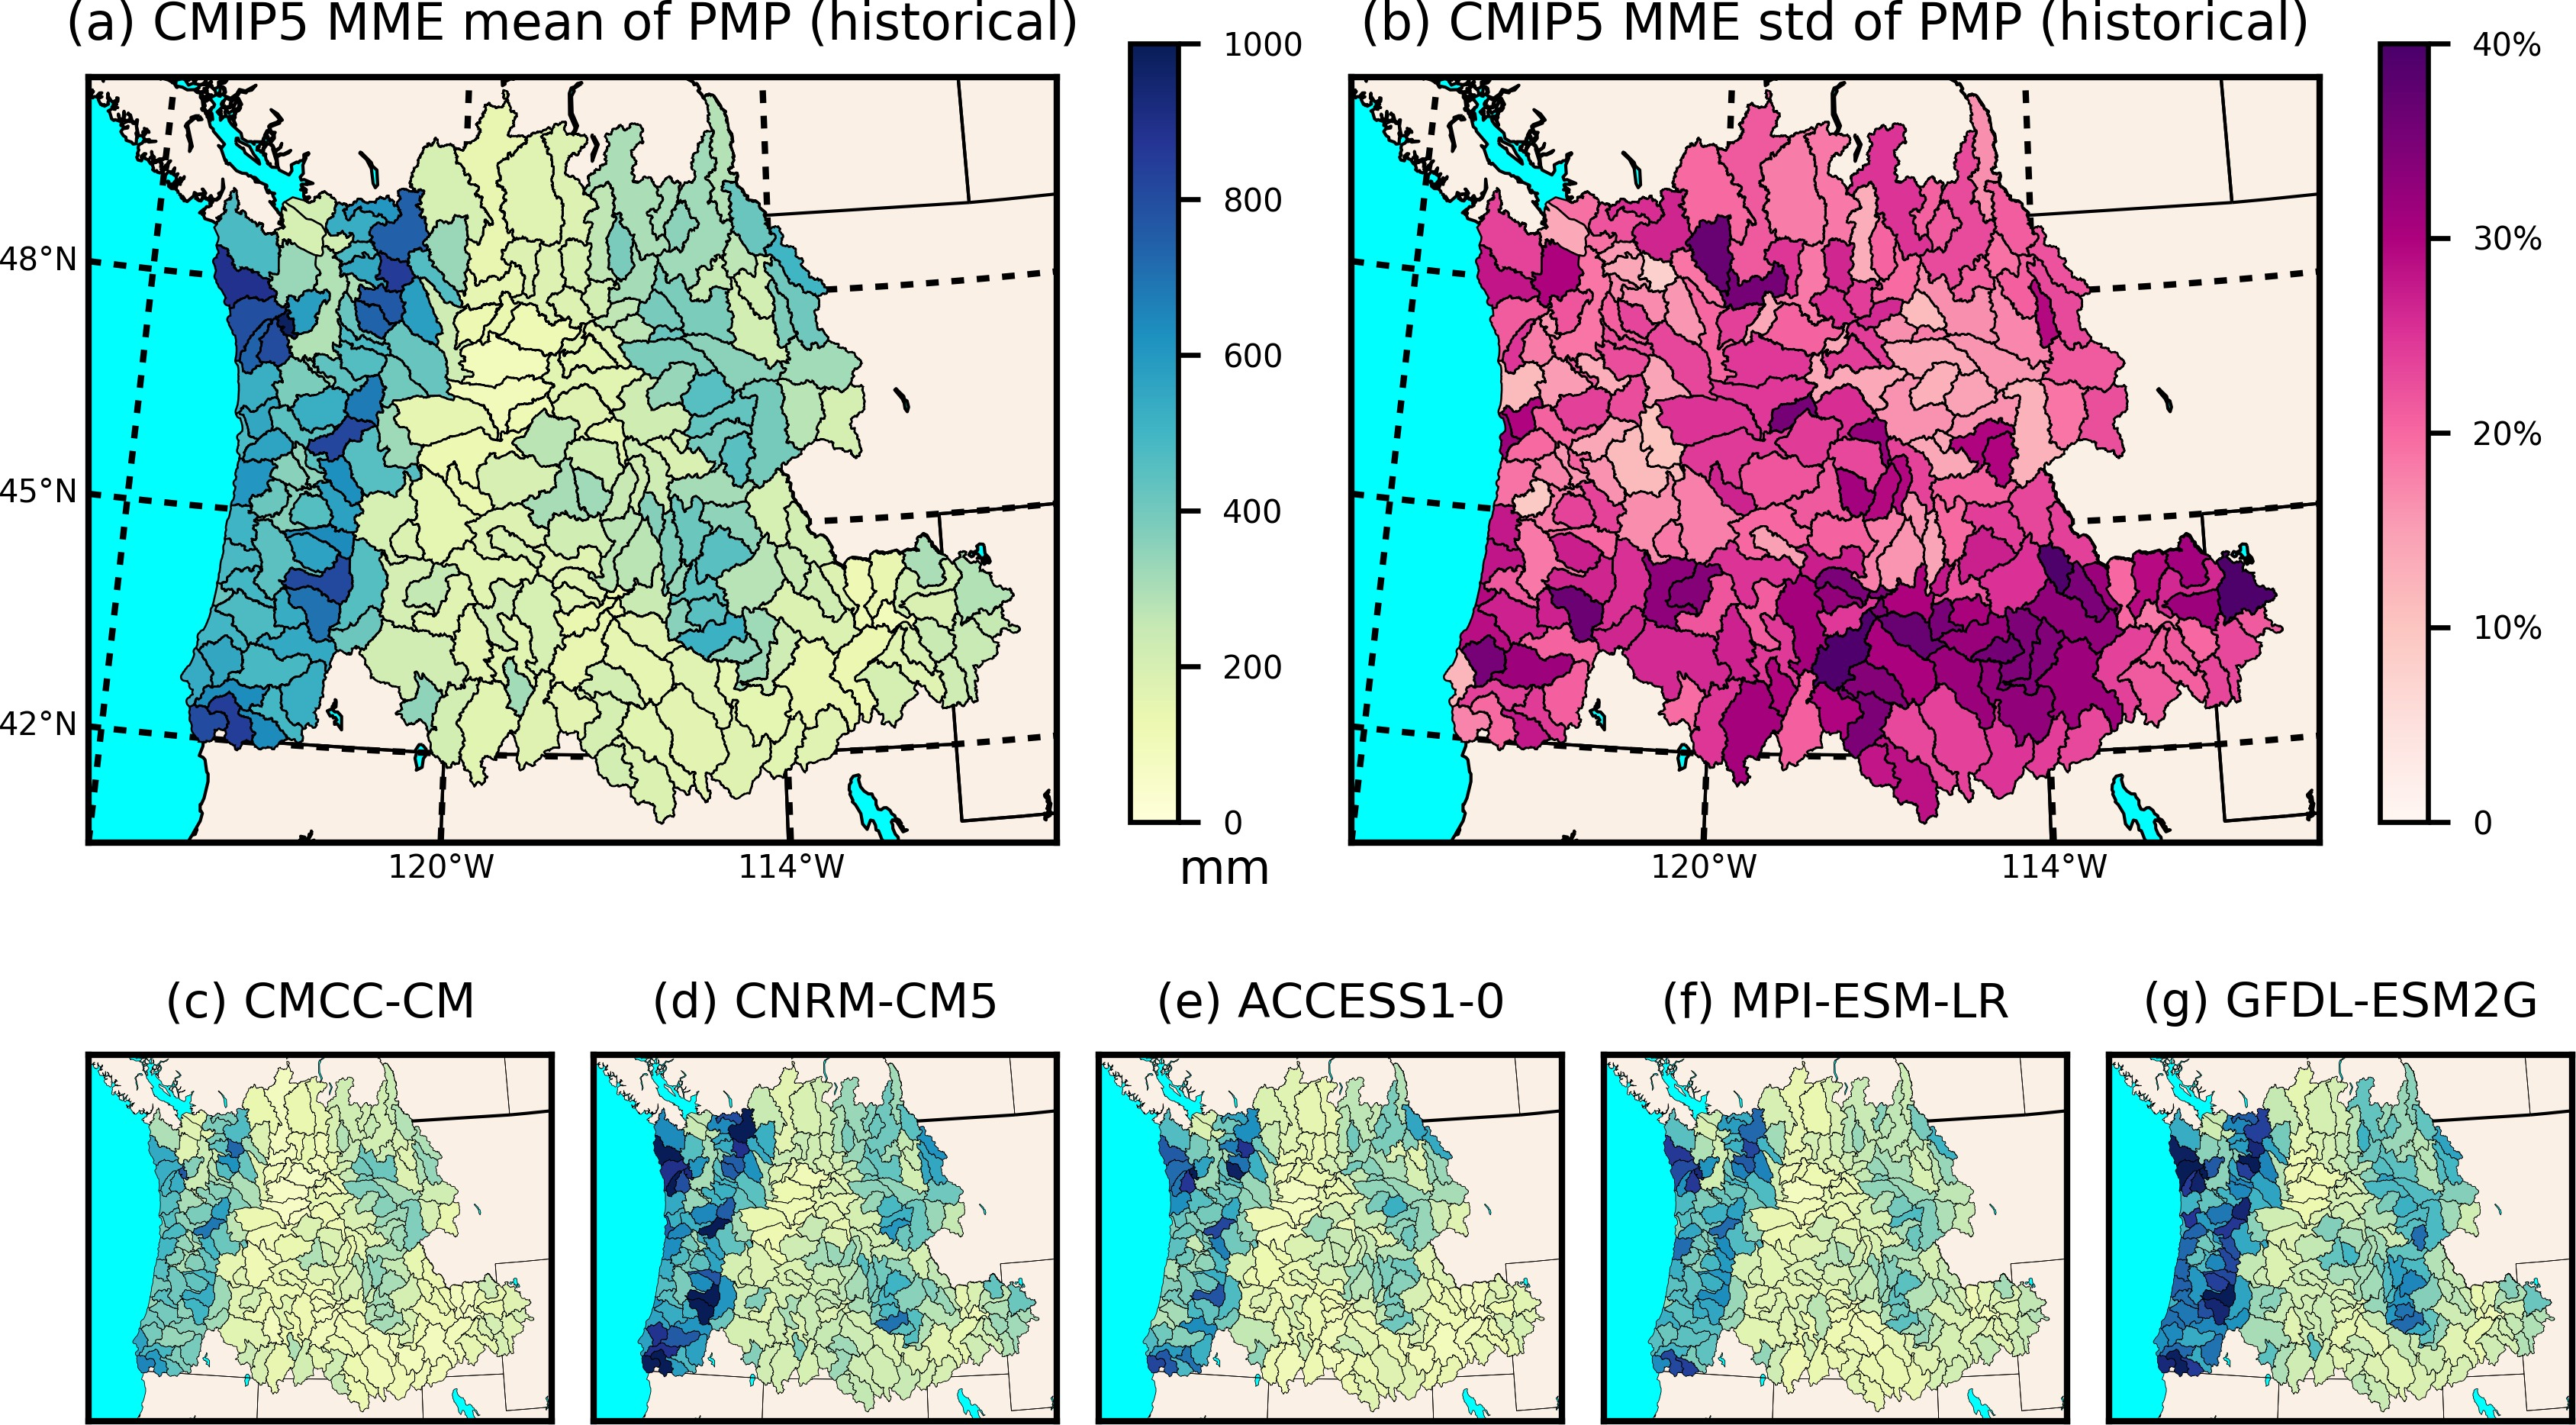
\includegraphics[width=\linewidth]{pics/ch3/fig7.jpg}
	\caption{Maximum 3-day rainfall from simulation and observation (pre-1948). Panels (a,d,g,j) are the WRF simulation, panels (b,e,h,k) are the gauge observation from Livneh dataset. Panels (c,f,i,l) are the difference (WRF - obs). All the units are mm.}
	\label{fig:3-7}
\end{figure}

For storms after 1979, the simulated maximum 3-day rainfall maps share the same patterns as observations (Figure \ref{fig:3-5}). In the 1997-CA event, the most rainy area is within the American River basin, and the model gives the correct 3-day rainfall peak as 450$\scriptsize{\sim}$500mm. In this event and 1982-CA event, the rain bands are along the Sierra Nevada. In both events, the model tends to overestimate rainfall in the southern part of Sierra Nevada, as indicated by the blue area in panels \ref{fig:3-5}(c) and \ref{fig:3-5}(f). In the 1980-PNW event, the north-south rain bands are captured by the model, both along the Pacific coast and along the Cascade. The model underestimates the rainfall in the coastal area, but overestimates in the Cascade region. Heavy rain area (3-day rainfall $>$ 240mm) are correctly captured in the Olympia peninsula and north Washington.

In the reconstruction of storms between 1948 and 1979 (Figure \ref{fig:3-6}), the storm patterns were not captured as precisely as was possible by WRF for the post-1979 storms. In the 1973-OK event, the heavy rainy area in the north Oklahoma and east Kansas are reflected in the simulation, although WRF model produces an overestimated continuous peak rainfall band in the east of Kansas. In the 1970-UT event, WRF simulations yield two separate rainy areas, one in middle Arizona, and one in southwest Colorado. This is in agreement with the observation. However, the model fails to reconstruct the heavy rainfall in the Colorado center. In the 1964-PNW event reconstruction, WRF successfully estimates the rainfall amount in the storm center, which is located at the US-Canada border. Observed storm center is to the south of the simulated one, though their area is quite similar. This means that the total rainfall, and the distribution of rainfall intensities are well captured, and we will check this later.

For 4 storms before 1948, the quality of model reconstruction varies (Figure \ref{fig:3-7}). The 1943-CA event is one of the best simulated cases of these 10 big storms. Two rain bands are well described by the model: the northeast one centered at Sierra Nevada, and the south one centered to the east of Los Angeles. Model overestimates the rain in the mountain area, but underestimates rainfall amount in the southern plain. The 1939-CA simulation is the worst reconstruction among the 10 cases. WRF fails to capture the rainy area to the east of the city of Los Angeles (panel \ref{fig:3-7}e), and the south-north rainfall gradient is not captured. The situation is similar for the 1930-NM storm, where the model underestimates the rainfall in the entire storm domain. In the 1929-AL event, however, the situation is a little different. The simulated storm is at middle Tennessee, while the observation indicates the storm center at southern Alabama. The maximum 3-day rainfall from the simulation is merely over 200mm, which is far less than the observed 280mm peak.

Figure \ref{fig:3-8} presents the histograms of daily rainfall intensities from both simulations and observations. To make it clear, lines are shown instead of histogram bins. In these 10 panels, red lines represent the best WRF simulations, and blue lines are from Livneh dataset. It is clear that if we do not take into account the information on the grids location and temporal structure, the model reconstructions are able to give reasonable description of daily rainfall evolution. The model results are closer to the observations in the light rainy area (daily rainfall$<$100mm). As shown in the panels \ref{fig:3-6}(g) and \ref{fig:3-6}(h), the size and magnitude of the simulated 1964-PNW storm center is quite similar to the observed center, though their locations are slightly different. If we do not account for the location shift, the ``1964-PNW" panel in Figure \ref{fig:3-8} suggests that model reconstruction captures the daily rainfall intensity accurately. The area of both light rainy grids and heavy rainy grids match the statistics from observation. Figure \ref{fig:3-8} also suggests that for most cases (except for the 1970-UT and 1929-AL storms), WRF successfully captures the highest daily rainfall, and in most case WRF tends to overestimate the heavy rain area. This makes the model estimates on the safe side in terms of potential damages caused by the storms.

\begin{sidewaysfigure}[htbp]
	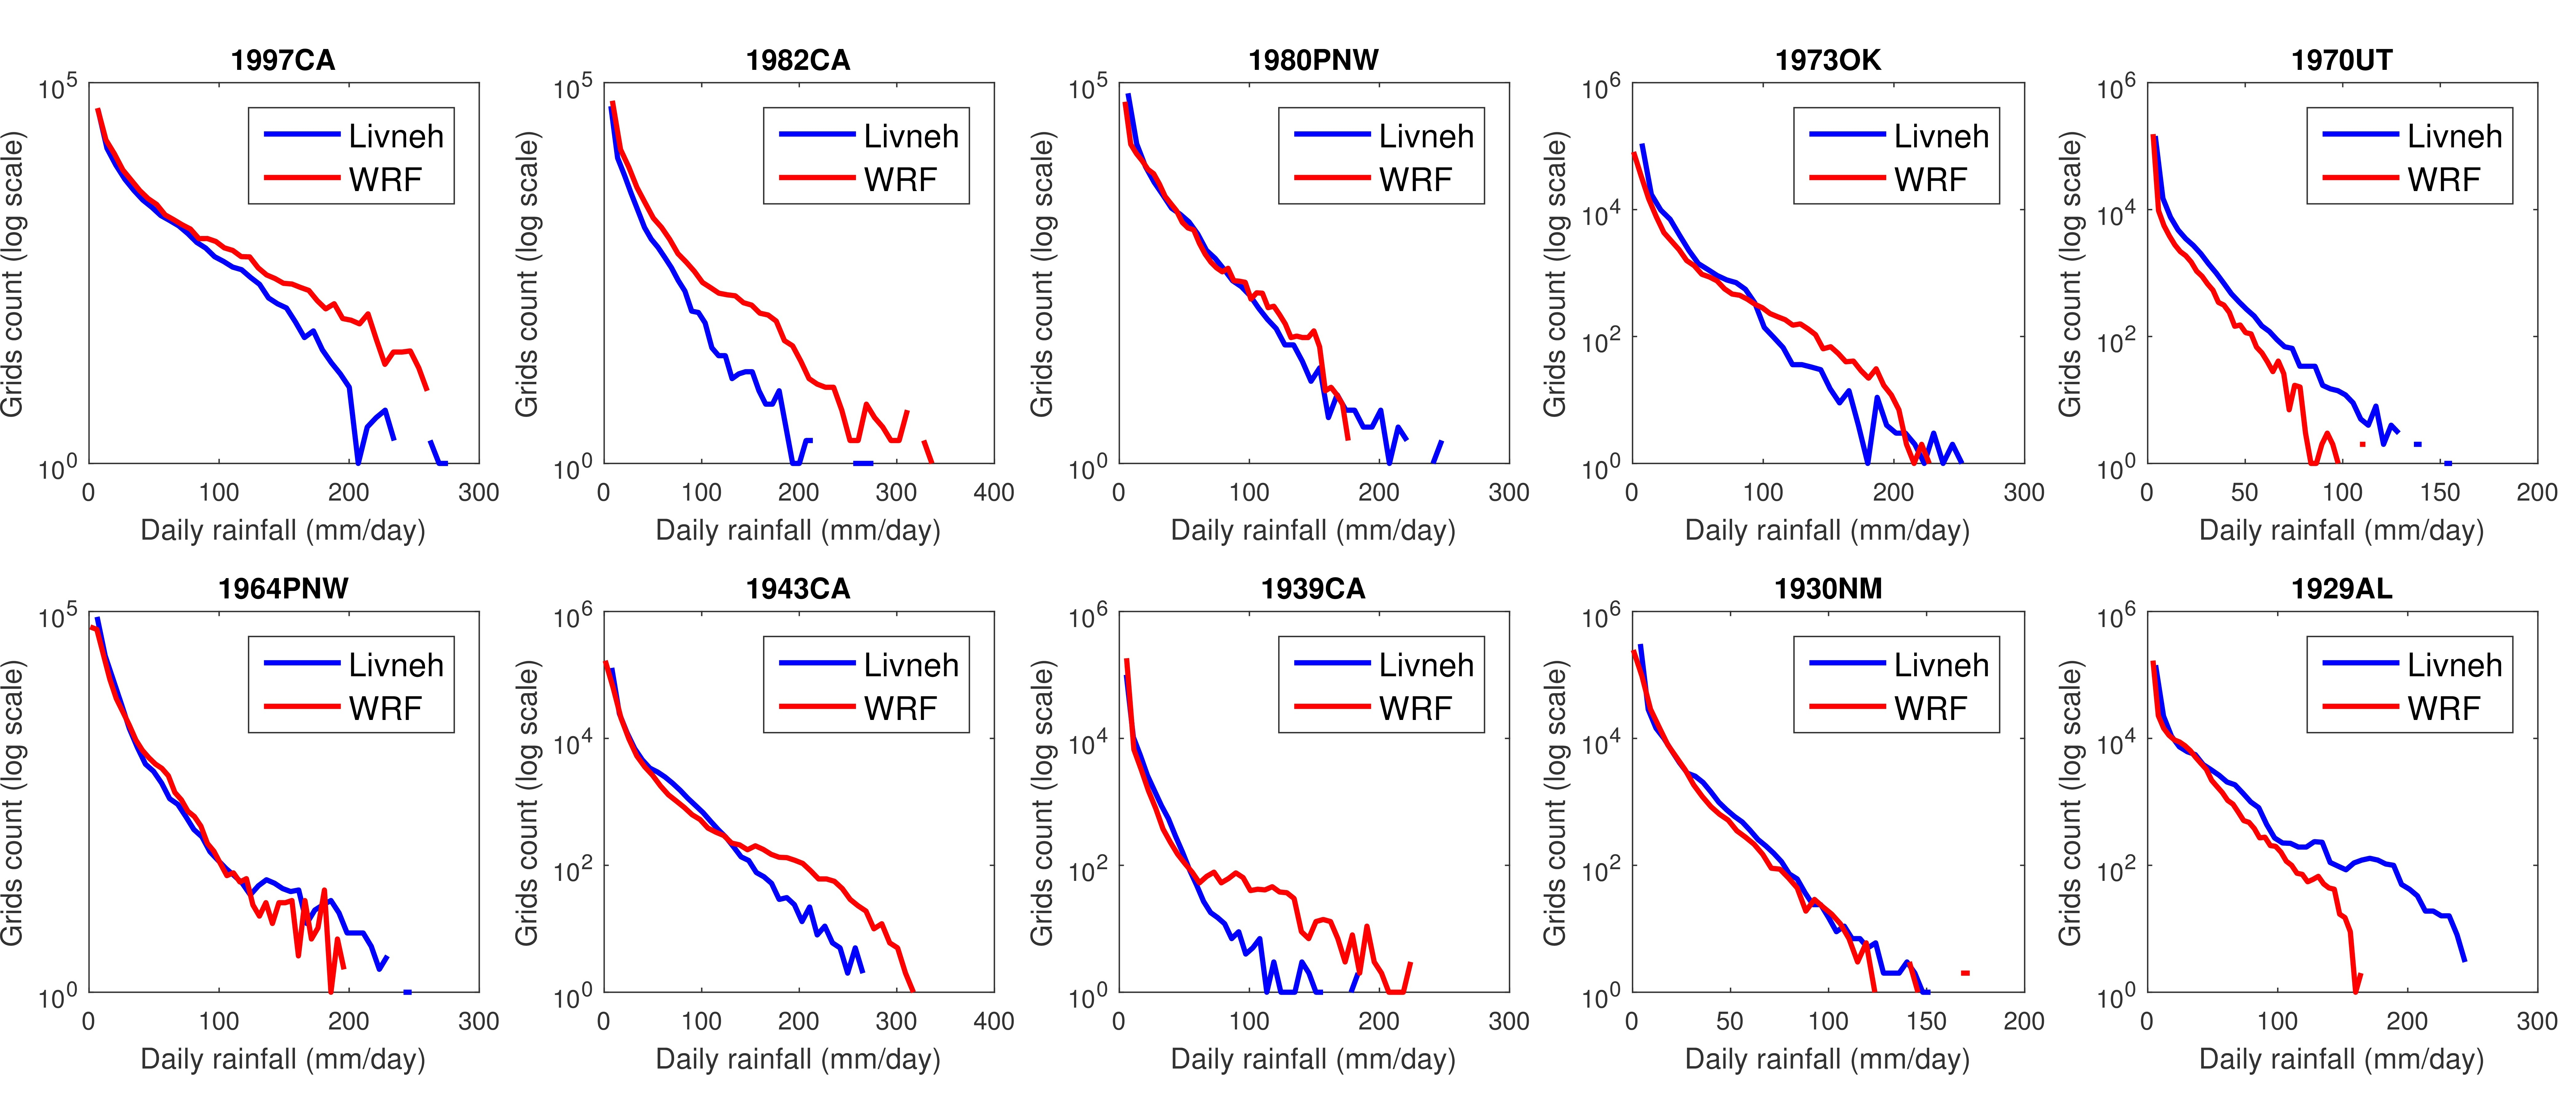
\includegraphics[width=\linewidth]{pics/ch3/fig8.jpg}
	\caption{Histogram of daily rainfall intensity from simulations and observations. Y-axis is on logarithmic scale.}
	\label{fig:3-8}
\end{sidewaysfigure}


\section{Discussion}

\subsection{WRF configuration for big storm simulation}

As shown in the results section, there is no single best (microphysics or cumulus) parameterization scheme that outperforms others in the simulation. Thus, it is necessary to take into consideration their possible combinations as a potential ‘ensemble’. This is in agreement with previous studies [\textit{Hasan}, 2014].

As shown in figures \ref{fig:3-2} and \ref{fig:3-3}, the model performance is mostly sensitive to the choice of IC/BC. Despite the differences caused by microphysics and cumulus schemes, simulations using NCEP2 IC/BC produce best results. Simulations using NNRP IC/BC yield acceptable result, which suggests that NNRP is also a suitable option for historical big storm reconstruction. This extends the CONUS storms that we can potentially reconstruct back to year 1948. It is in agreement with previous studies [\textit{Tan}, 2010] where the storms in the American River basin since 1951 were well simulated using NNRP IC/BC. In our study, the area that is feasible for numerical approach was expanded to the whole CONUS.

The best combinations for each storm are shown in table \ref{table:3-2}. It is obvious that though the specific best ones are somewhat different, most storms benefit from Morrison microphysics scheme and KF cumulus scheme. Also as table \ref{table:3-2} suggests, finer resolution does not always help to improve the simulation quality. Based on the results of these 10 storms, we recommend the Morrison microphysics, KF cumulus scheme and a relatively coarser grid (such as 15km grids) as the starting set of options of the modeling attempts on other storms over CONUS. This is in agreement with study of \textit{Chen et al.} [2017], where KF cumulus and Morrison microphysics were also recommended as starting options for extreme storm simulations based on the experiment with 2010 May Nashville, TN storm. Therefore, it looks like an optimal combination exists for different types of storms over CONUS, although more experiments are required to confirm it.

\subsection{Are we ready to reconstruct old storms for assessing future engineering safety?}

Figures \ref{fig:3-2} and \ref{fig:3-3} suggest that we are now able to reconstruct the big storms after 1940s. For these storms, the simulated rainfall distributions (both spatial and statistical) are in good agreement with observations. The quality of these simulations makes WRF-reconstruction suitable for further studies, such as the model-based PMP estimation or storm maximization [\textit{Tan}, 2010; \textit{Stratz and Hossain}, 2014], and exploring sensitivity of PMP to the land cover/land use change, global warming and other anthropogenic drivers.

For storms before 1948, current results suggest that there might be some chances to get a good reconstruction. In the ``1930-NM" panel of figure \ref{fig:3-8}, the simulated and observed daily rainfall are matched surprisingly well in the frequency space. But as the maps in panels \ref{fig:3-7}(g) and \ref{fig:3-7}(h) suggest, this reconstruction fails to give out the spatial information. Thus such reconstruction is not usable for engineering purposes yet.

\subsection{Is 20CR suitable for single event reconstruction?}

20CR product has been widely used, and has shown its power in the climate studies in various parts of the world. For example, \textit{Kong and Bi} [2015] used 20CR and WRF model to study the mean climatic characteristics in China over 1981-2010, and concluded that 20CR input is able to produce main features in surface air temperature and precipitation at seasonal scale. Here we attempted to use 20CR in single event simulations. Results suggest that for the 1943-CA storm, WRF can reconstruct fairly accurately the storm structure, with evaluation results comparable to the storms of the 1970s. However, for other storms prior to 1948, the simulation quality quickly drops. In the 1939-CA and 1930-NM events simulation, it fails to produce the correct storm areas, and the simulated storm characteristics are inaccurate. In the 1929-AL event the simulated rainfall is completely to the north of the actual rainfall area. While it may be possible to use these results for the estimation of storm duration-area-intensity relationship, such bias in the results makes them unsuitable for studies that check the impact of local land use change on this storm or consequential probable maximum flood (PMF) analyses.

In general, 20CR is not yet ready for single storm event simulation for storms prior to 1948. This currently holds back our ability to numerically reconstruct the historical big storms at prior to that period. Given the ability to represent the annual and seasonal climate characteristics reasonably well, it would be good to conduct some investigation and find out when in time the rainfall statistics of 20CR become no longer comparable to observations.


\section{Conclusions}

In this chapter we evaluated the performance of numerical atmospheric models in reconstructing 10 big storms over CONUS during 1920-2000. Our ability to reconstruct past extreme storms will dictate how well we can understand such storms may evolve in future for assessing water infrastructure safety. Using the gauge observation data as reference, we evaluated the reconstruction qualities on the spatial coverage of rainy area, the correlations between simulated and observed maximum rainfall in different periods. The main results are:

(1) Model reconstruction is most sensitive to the choices of initial/boundary conditions. Therefore, reconstruction of historical big storms is restricted by the availability of the initial/boundary conditions;

(2) We are able to reconstruct the big storms after 1948, using carefully chosen initial/boundary conditions. The spatial patterns of these big storms are well captured by the model;

(3) The storm characteristics, presented by the maximum daily, 2-day and 3-day rainfall, can be well captured by the numerical models. Models tend to slightly overestimate the heavy rainy area, and this puts the constructed rainfall maps on the safe side in the engineering practices;

(4) Twentieth Century Reanalysis (20CR) Product, one of the very few available choices of IC/BC to simulate storms before the 1948, is not yet ready for single extreme event studies. 

As we look into the future of sustainable supply of water and protection against hazards, we need to contend with the state of our extensive water management infrastructure that were built using historical records and approaches that do not provide future insights. To gain this insight into the future as to how design-class extreme storms may behave in the future given changes to land cover and a warming atmosphere, it is important that we understand how well past storms can be physically reconstructed. This study provided a platform for storm reconstruction of the last 100 years’ extreme storms using a numerical modeling framework that we can now use for estimating future design parameters for water infrastructure safety such as PMP and PMF under a future scenario of change.

